\documentclass[../main-report.tex]{subfiles}
\begin{document}

\section{Hiện thực}
\subsection{Môi trường hiện thực}
Để thuận tiện trong việc đóng gói và triển khai ứng dụng, nhóm tác giả sử dụng công nghệ Container để hỗ trợ, đại diện tiêu biểu cho công nghệ Container mà nhóm tác giả chọn để sử dụng là Docker\footnote{https://www.docker.com}.

Công nghệ Docker container giúp người phát triển có thể triển khai ứng dụng ở bất kì đâu miễn là thiết bị đó có thể chạy được docker. Các ứng dụng được đóng gói trong container, có thể kiểm tra, xóa bất kì container nào. Các ứng dụng được triển khai dễ dàng và đồng nhất giữa các môi trường khác nhau.

Phiên bản docker và ứng dụng kèm theo mà nhóm tác giả triển khai bao gồm:

\begin{itemize}
\item \textbf{Docker Engine:} 19.03.3
\item \textbf{Docker Compose}: 1.21.0
\end{itemize}

\subsection{Các công nghệ được sử dụng}
Dựa vào kiến trúc hệ thống ở hình \ref{fig:system-architecture}, nhóm tác giả tiến hành chọn các công nghệ để hiện thực. Sơ đồ tổng quan về các công nghệ mà nhóm tác giả hiện thực được thể hiện ở hình \ref{fig:architecture-implementation}.

\begin{figure}[ht!]
\begin{center}
\label{fig:architecture-implementation}
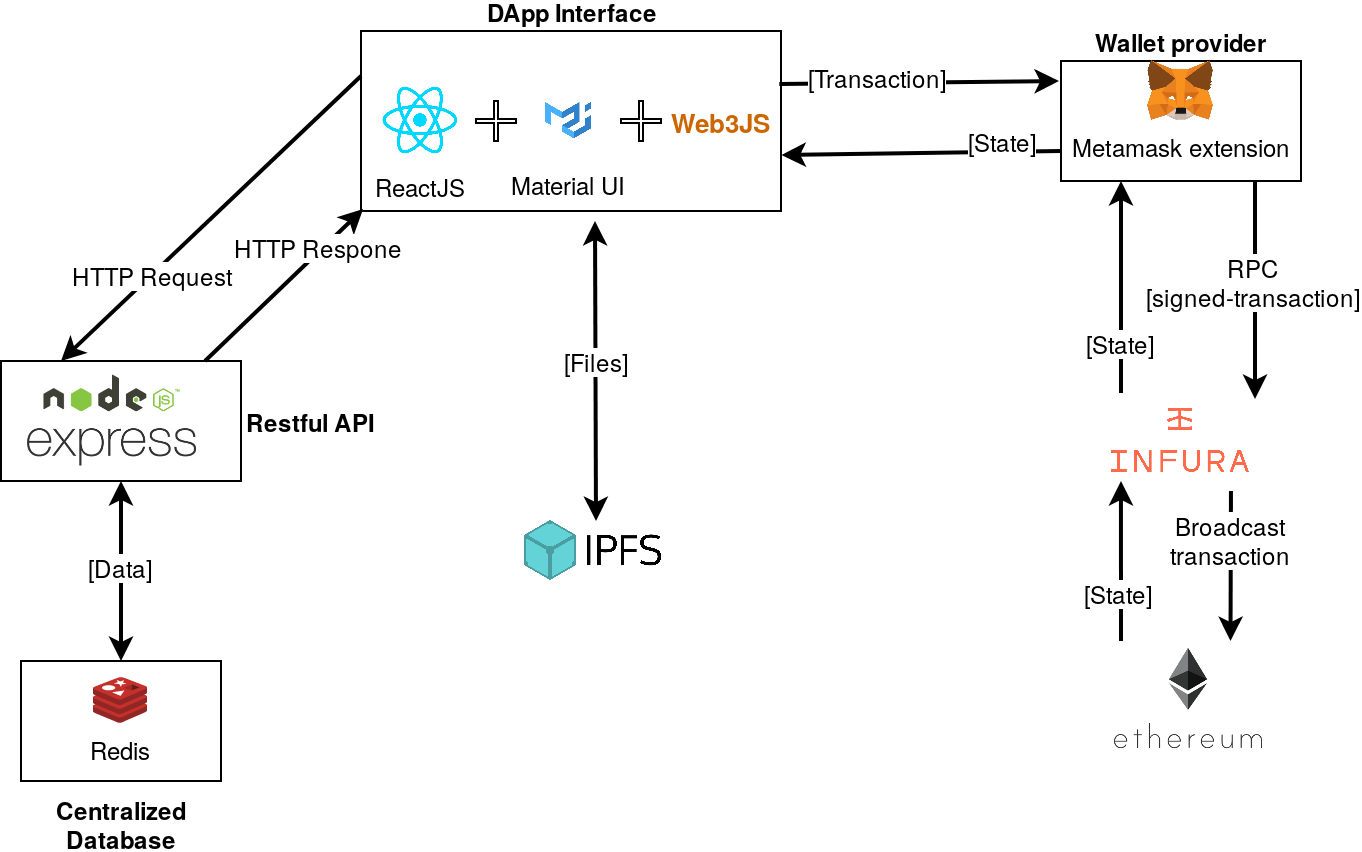
\includegraphics[scale=0.3]{architecture-implementation}
\caption{Sơ đồ hiện thực hệ thống}
\end{center}
\end{figure}

Các công nghệ được sử dụng bao gồm:
\begin{itemize}
\item Phần giao diện người dùng (\gls{frontend}): nhóm tác giả sử dụng \textbf{ReactJS/NodeJS} kết hợp \textbf{Material UI} để tạo giao diện ứng dụng web cho người dùng. Để tương tác với các hợp đồng thông minh, nhóm tác giả sử dụng thư viện Web3js và trình mở rộng Ví Metamask.
\item Phần \gls{backend} được chia làm hai thành phần như sau:
\begin{itemize}
 \item Kiến trúc phi tập trung (decentralized): nhóm sử dụng ngôn ngữ solidity để xây dựng các \gls{smartcontract} kết hợp \acrshort{ipfs} để thực hiện lưu trữ các dữ liệu phi tập trung.
 \item Kiến trúc tập trung (centralized): công nghệ NodeJS kết hợp với Redis để tổ chức và tương tác với dữ liệu tập trung.
 \end{itemize} 
\end{itemize}

Với hợp đồng thông minh và ngôn ngữ Solidity, nhóm tác giả sử dụng bộ công cụ Truffle framework để xây dựng và triển khai các mã hợp đồng thông minh.

\subsubsection{Công nghệ ReactJS/NodeJS}
\textbf{ReactJS} là một thư viện để hỗ trợ cho việc phát triển giao diện của người dùng. Đây là một trong những thư viện \gls{frontend} nổi tiếng với hơn $141.000$ sao đánh giá với hơn 2.8 triệu người dùng trên dịch vụ lưu trữ mã nguồn Github\footnote{https://github.com} (số liệu cập nhật tháng 12 năm 2019). Thư viện này được hỗ trợ và phát triển bởi Facebook\footnote{https://www.facebook.com} và Instagram\footnote{https://www.instagram.com} cùng với cộng đồng các nhà phát triển trên toàn thế giới và đang được phát triển từng ngày. ReactJS cung cấp tốt hơn về trải nghiệm người dùng và đồng thời có nhiều thư viện bên thứ ba hữu ích khác được phát triển kèm theo.

ReactJS được thiết kế và phát triển theo kiến trúc các component\footnote{là một kiểu kiến trúc trong phát triển phần mềm, chia ứng dụng ra thành các thành phần, bộ phận không phụ thuộc lẫn nhau và có thể tải sử dụng các thành phần này khi cần thiết}. Theo như tài liệu từ Facebook, định nghĩa React là một thư viện dành cho phát triển các mô đun cho giao diện người dùng. Về cơ bản, React cho phép các nhà lập trình phát triển các ứng dụng web lớn, phức tạp và đổng thời có thể thay đổi dữ liệu mà không cần tải lại trang. React sử dụng DOM ảo, điều này có tác dụng tăng hiệu suất kết xuất trang web, đồng thời nâng cao trải nghiệm của người dùng, cũng như rất dễ dàng lập trình phát triển sản phẩm.

\textbf{Node.js} hay còn được gọi là \textbf{Node} – là một nền tảng chạy trên môi trường Javascript hay còn được gọi là một nền tảng chạy trên môi trường V8 JavaScript runtime. Công nghệ V8 đã được triển khai hầu hết ở C và C++, công nghệ này tập trung chủ yếu vào hiệu suất và ít tiêu tốn bộ nhớ. Hầu hết V8 hỗ trợ chủ yếu Javascript trên trình duyệt (chú ý nhất là Google Chrome), mục đích hỗ trợ của Node đó chính là hỗ trợ các tiến trình có thời gian chạy dài. Không giống như những ngôn ngữ khác, Node không hỗ trợ đa luồng, nhưng hỗ trợ xử lý bất đồng bộ \cite{nodejs-performance}. Nhờ vào tính năng xử lý bất đồng bộ này, Node còn được biết đến là một nền tảng xử lý nhanh chóng hàng ngàn yêu cầu đồng thời, chịu tải cao, tốc độ thực thi và khả năng mở rộng tốt.

Đánh giá về hiệu suất của các ứng dụng chạy Node.js, nhóm tác giả có tham khảo nghiên cứu của tác giả Robert Ryan McCune về đo lường hiệu suất của ứng dụng Node.js \cite{mccune2011node}. Trong bài nghiên cứu, tác giả Robert Ryan McCune đã thực hiện phần đánh giá trên một máy ảo \textbf{Ubuntu 11.10} được tạo bởi VMWare Fusion 4.0.2 trên iMac \textit{OS X 10.6.8} với 8GB RAM và \textit{3.06Ghz Intel Core 2 Duo}, máy ảo này được được cấu hình với bộ nhớ là \textbf{2GB RAM}, và một bộ vi xử lý lõi kép. Tác giả đã thực hiện đồng thời 100 và 1000 yêu cầu đến máy chủ chạy bằng Node và thu được kết quả là thời gian trả lời từ máy chủ chưa tới 70ms. Tương tự thực hiện 500 yêu cầu đồng thời và thực hiện tổng cộng 10.000 yêu cầu thì thời gian phản hồi là dưới 140ms.

\subsubsection{Material UI framework}
\textbf{Material UI} là một thư viện được \textit{Google}\footnote{https://www.google.com} viết dành riêng cho ReactJS, bao gồm tập hợp nhiều các thành phần được xây dựng và thiết kế theo phong cách Material. Với hơn 52.8 nghìn sao đánh giá trên cộng đồng Github, và được sử dụng bởi hơn 139.000 dự án khác nhau, Material là một trong những thư viện UI được nhiều người sử dụng nhất trên thế giới. Giao diện của Material cũng tương đồng với các sản phẩm của Google như: \textit{Gmail, Google tìm kiếm, Google Form},\ldots

Material UI hiện tại cũng đang được sử dụng bởi \textit{NASA, UNIQLO, shutterstock},\ldots

Trong cuộc khảo sát vào năm 2019 của Oliver được đăng trên trang Medium\footnote{Nguồn: https://medium.com/material-ui/2019-material-ui-developer-survey-results-c9589434bbcf} đã chỉ ra rằng, có đến 74.4\% của 734 người khảo sát cho rằng sẽ thất vọng khi không còn sử dụng thư viện này. Biểu đồ thể hiện thái độ người khảo sát khi không còn được sử dụng thư viện Material ở hình \ref{fig:material-chart-survey}.

\begin{figure}[ht!]
\begin{center}
\label{fig:material-chart-survey}
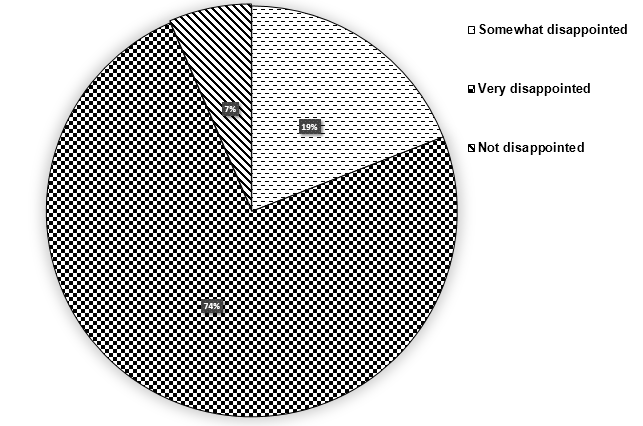
\includegraphics[scale=0.8]{material-chart-survey}
\caption{Biểu đồ thể hiện thái độ người dùng khi không được sử dụng thư viện Material}
\end{center}
\end{figure}

Cũng tại bài viết, tác giả đã ghi nhận nhận những lợi ích từ người khảo sát cho rằng yếu tố tập trung vào luồng xử lý, tiết kiệm thời gian, dễ dùng, \ldots và có đến 70\% dùng thư viện này để xây dựng dashboard, 40\% để thiết kế hệ thống, 35\% dùng để thiết kế các trang doanh nghiệp.

\subsubsection{Cơ sở dữ liệu Redis}
\textbf{Redis} là một cơ sở dữ liệu thường được xếp vào nhóm cơ sở dữ liệu NoSQL, được phát triển vào năm 2009. Khác với những cơ sở dữ liệu khác, Redis lưu dữ liệu trên RAM của máy chủ, điều này làm cho việc truy xuất giá trị nhanh hơn so với cách lưu trữ truyền thống – lưu trữ trên ổ cứng. Sau một thời gian, các bản ghi được lưu trên RAM này sẽ được lưu xuống ổ cứng nhằm tiết kiệm tài nguyên bộ nhớ RAM.

Các đặc điểm của Redis \cite{6106531}:

\begin{enumerate}[label=(\roman*)]
\item Redis là một dạng lưu trữ dữ liệu \textit{key-value}, như được nói ở trên khi Redis chạy, dữ liệu sẽ được lưu trữ trong bộ nhớ, do đó nó có thể xử lý hơn 100.000 thao tác đọc và ghi mỗi giây.
\item Redis hỗ trợ nhiều dạng lưu trữ như \textit{List} và \textit{Set},\ldots
\item Giá trị lớn nhất lưu trên Redis là 1GB.
\item Nhược điểm của Redis là dung lượng của cơ sở dữ liệu bị giới hạn bởi bộ nhớ vật lý, do đó Redis không nên dùng làm cơ sở dữ liệu cho các dự án lớn và khả năng mở rộng kém.
\end{enumerate}

Với các đặc điểm trên, Redis phù hợp cho việc cung cấp hiệu suất cao cho lượng dữ liệu nhỏ.

\subsubsection{IPFS}
\textbf{\acrfull{ipfs}} là một giao thức chia sẻ tệp tin được phân tán ngang hàng \acrfull{p2p}. Giao thức này cho phép người dùng chia sẻ các tệp tin ngang hàng với nhau mà không cần có sự xuất hiện của máy chủ. Các dữ liệu khi người dùng tải lên sẽ được băm ra và đồng thời sinh ra mã băm của dữ liệu ấy. Với các dữ liệu giống nhau thì sẽ tạo ra những hàm băm giống nhau, do đó IPFS sẽ hạn chế được sự trùng lặp.
 
\acrshort{ipfs} có thể giải quyết vấn đề về lưu trữ dữ liệu lớn cho các ứng dụng \gls{blockchain} bằng cách sử dụng blockchain để lưu trữ địa chỉ của dữ liệu được ra bằng IPFS (chính là mã băm nhận diện cho tập tin) và đặt địa chỉ bất biến này cho một giao dịch trong blockchain. Không những giải quyết vấn đề lưu trữ, \acrshort{ipfs} còn giải quyết vấn đề về băng thông bằng cách phân tán nội dung đến hệ thống \acrshort{p2p}. Do đó, khi truy cập tập tin nào đó bằng cách dùng hàm băm, nút gần nhất với tệp sẽ phản hồi và gửi tệp cho người yêu cầu. Như đã được chứng minh từ trước \cite{5235364}, một hệ thống phân tán \acrshort{p2p} có thể tiết kiệm lên đến 60\% so với hệ thống truyền thống. Đồng thời, IPFS còn tăng tính bảo mật và chống lại các cuộc tấn công từ chối dịch vụ và giới hạn lại kiểm duyệt vì không có địa chỉ IP cụ thể của máy chủ bị chặn \cite{8441990}.

\subsubsection{Bộ công cụ Truffle framework}
\textbf{Truffle} là một bộ công cụ để phát triển các ứng dụng phi tập trung trên mạng Ethereum. Khi sử dụng truffle, theo tài liệu kĩ thuật\footnote{https://www.trufflesuite.com/docs} của Truffle mô tả framework này có các tính năng sau:

\begin{itemize}
\item Tích hợp các tính năng biên dịch, liên kết, triển khai và quản lý mã nhị phân các hợp đồng thông minh.
\item Tự động kiểm thử các contract để quá trình phát triển nhanh hơn.
\item Khung triển khai các hợp đồng thông minh có thể tùy biến và mở rộng.
\item Quản lí mạng để triển khai hợp đồng thông minh đến bất kì mạng công khai hay riêng tư nào.
\item Quản lí gói với EthPM và NPM, sử dụng tiêu chuẩn ERC190\footnote{https://github.com/ethereum/EIPs/issues/190}.
\item Tương tác trực tiếp với hợp đồng thông minh thông qua giao diện console.
\end{itemize}

\subsubsection{Thư viện web3js}
\textbf{Web3js} là một thư viện được viết bằng \textit{Javascript}, thư viện cung cấp các API cần thiết cho lập trình viên tương tác với mạng blockchain Ethereum cũng như là hợp đồng thông minh trên Ethereum thông qua giao tiếp \acrfull{rpc}\footnote{Remote Procedure Call (RPC) tạm dịch là các cuộc gọi thủ tục từ xa, đây là một phương pháp dùng để trao đổi dữ liệu theo kiến trúc yêu cầu - phản hồi.}.

Theo như tài liệu của thư viện Web3js\footnote{https://web3js.readthedocs.io}, các hàm trong \textit{web3-eth} dùng để tương tác với mạng blockchain và hợp đồng thông minh như là lấy thông tin địa chỉ của tài khoản, chọn lựa mạng,\ldots. \textit{web3-ssh} cung cấp giao thức để giao tiếp \acrshort{p2p} và broadcast. \textit{web3-bzz} được dành cho giao thức swarm\footnote{swarm - một mô hình kiến trúc phân tán.}, lưu trữ tập trung. Cuối cùng là \textit{web-utils} chứa đựng các hàm tiện ích cho dự án DApp.
\subsubsection{Ví Metamask}
\textbf{Metamask}\footnote{https://metamask.io} là một ví Ethereum, được phát triển dưới dạng trình mở rộng trên trình duyệt. Metamask là ứng dụng cầu nối cho phép người dùng truy cập vào các ứng dụng web phi tập trung và tương tác với mạng blockchain đơn giản hơn mà không cần phải chạy một nút Ethereum đầy đủ.

Metamask cung cấp giao diện người dùng để quản lí các khóa bí mật, các giao dịch, số dư Ethereum, kí transaction, \ldots. Metamask có giao diện dễ dùng, hỗ trợ hầu hết các trình duyệt hiện nay.
\subsection{Các bước hiện thực}
Phần hiện thực hệ thống được viết thành kịch bản và thực hiện tự động bằng trình Docker Compose, hệ thống sẽ được chia thành nhiều dịch vụ, bao gồm:

\begin{itemize}
\item \textbf{smartcontract} -- thực hiện chức năng biên dịch và triển khai các hợp đồng thông minh lên mạng blockchain, sau đó trả về các tệp json chứa \acrfull{abi}\footnote{là cách tiêu chuẩn để tương tác với các hợp đồng trong hệ sinh thái Ethereum, cả từ bên ngoài blockchain và cho tương tác giữa các hợp đồng với nhau.} và địa chỉ của hợp đồng thông minh. Các tệp json này được \gls{frontend} sử dụng để kết nối với hợp đồng thông minh.
\item \textbf{client} -- kết xuất và triển khai giao diện người dùng.
\item \textbf{store\_centralized\_data} -- xây dựng và triển khai Restful API để xử lí đọc và ghi dữ liệu ở cơ sở dữ liệu tập trung.
\item \textbf{redis} -- cơ sở dữ liệu Redis, lưu trữ các thông tin mô tả về chiến dịch.
\end{itemize}

Nội dung tệp \textbf{docker-compose.yml}\footnote{docker-compose.yml là tệp mặc định được sử dụng bởi Docker Compose} triển khai các dịch vụ trong hệ thống như sau:

\begin{lstlisting}
version: '3.4'
services:
  smartcontracts:
    build: ./smartcontracts/
    volumes:
      - contracts:/app/build/
  client:
    build: ./client/
    ports:
      - 3000:3000
    volumes:
      - ./client/src/:/app/src/
      - contracts:/app/src/contracts/:ro
    depends_on:
      - smartcontracts
  store_centralized_data:
    build: ./store_centralized_data/
    ports:
      - 8080:8080
    volumes:
      - ./store_centralized_data/src/:/app/src/
    depends_on:
      - redis
  redis:
    image: redis:alpine
    command: redis-server --requirepass 12345678 --appendonly yes
    volumes:
      - data:/data
volumes:
  data:
  contracts:
\end{lstlisting}

Các bước để hiện thực hệ thống như sau:

\begin{itemize}
\item \textbf{Bước 1:} cấu hình thông số các \gls{service}.
\item \textbf{Bước 2:} tạo các \gls{service}.
\item \textbf{Bước 3:} chạy các \gls{service}.
\end{itemize}

Chi tiết các bước trên được mô tả ở mục \ref{sec:configure-service}, \ref{sec:build-service}, \ref{sec:run-service}.

\subsubsection{Cấu hình thông số các service}
\label{sec:configure-service}
Để các service chạy chính xác, nhóm tác giả tạo ra các biến môi trường được lưu ở file \textbf{.env} trong thư mục của từng service trong bộ mã nguồn chương trình kèm theo khóa luận này để phục vụ cho việc cấu hình.

Cấu hình service smartcontracts, chỉnh sửa các biến sau trong tệp \textbf{smartcontracts/.env}:

\begin{itemize}
\item \texttt{MNEMONIC} -- biến chứa giá trị mnemonic của tài khoản nhân viên vận hành hệ thống, mnemonic là một chuỗi 12 kí tự gợi nhớ, chuỗi này gắn liền với các tài khoản trên ethereum. Tài khoản mặc định gắn với mnemonic nhập vào sẽ là tài khoản triển khai các hợp đồng thông minh lên mạng blockchain.
\item \texttt{INFURA\_API\_KEY} -- khóa để sử dụng API của Infura\footnote{https://infura.io} để tương tác với một nút trong mạng blockchain để triển khai các hợp đồng thông minh lên mạng. Để có khóa này, có thể đăng kí sử dụng API của Infura. Giá trị mặc định: 

\begin{lstlisting}
417dc4db619c43798109b08709985882
\end{lstlisting}
\end{itemize}

Cấu hình service client, chỉnh sửa các biến trong tệp \textbf{client/.env}:

\begin{itemize}
\item \texttt{REACT\_APP\_STORE\_CENTRALIZED\_API}  -- là địa chỉ máy chủ Restful API trong mô hình hệ thống, định dạng \textit{``http://[IP|DOMAIN]:PORT/''}
\item \texttt{REACT\_APP\_DEFAULT\_NETWORK} -- địa chỉ để kết nối đến một nút mạng blockchain mặc định để lấy dữ liệu, phục vụ việc hiển thị thông tin chiến dịch khi không có ví Metamask. Giá trị mặc định:

\begin{lstlisting}
https://ropsten.infura.io/v3/b56a34eee35e491691629e3412875afa
\end{lstlisting}

\item \texttt{REACT\_APP\_RECAPTCHA\_ENABLE} -- biến cờ để xác định việc sử dụng captcha trong trang đăng kí chiến dịch. Với giá trị \textbf{``1''} là xác định sử dụng dịch vụ captcha, \textbf{``0''} là tắt captcha. Giá trị mặc định: \textbf{``0''}.
\item \texttt{REACT\_APP\_RECAPTCHA\_SITEKEY} -- phần captcha trên trang đăng kí chiến dịch được nhóm tác giả sử dụng là \textbf{reCAPTCHA}\footnote{https://www.google.com/recaptcha/intro/v3.html} của \textit{Google}, nên để sử dụng được thành phần này trong hệ thống, cần đăng kí dịch vụ ReCaptcha của Google. Sau đó thực hiện lấy khóa captcha tương ứng để sử dụng. Nếu captcha không được sử dụng thì có thể bỏ qua biến này.
\end{itemize}

Cuối cùng là cấu hình cho service \textbf{store\_centralized\_data}:

\begin{itemize}
\item \texttt{PORT\_LISTEN} -- cổng mà máy chủ sẽ lắng nghe. Giá trị mặc định: \textbf{``8080''}.
\item \texttt{RECAPTCHA\_ENABLE} -- biến cờ để xác định việc sử dụng captcha trong trang đăng kí chiến dịch. Với giá trị \textbf{``1''} là xác định sử dụng dụng dịch vụ captcha, \textbf{``0''} là tắt captcha. Giá trị mặc định: \textbf{``0''}.
\item \texttt{RECAPTCHA\_SECRET\_KEY} -- phần khóa captcha này liên kết với captcha ở phía service \textbf{client}. Tuy nhiên ở service này sẽ nhận kết quả captcha từ client gửi và xử lí. Nên khóa ở đây là khóa bí mật của dịch vụ \textit{reCAPTCHA}.
\item Các biến \texttt{REDIS\_HOST}, \texttt{REDIS\_PORT}, \texttt{REDIS\_PASSWORD} là thông tin để kết nối đến dịch vụ redis. Giá trị mặc định được gán cho các biến này gồm: ``redis'', ``6379'', ``12345678''.
\end{itemize}
\subsubsection{Tạo các service}
\label{sec:build-service}
Để các service có thể chạy được thì cần cài đặt môi trường và thư viện tương ứng. Để đơn giản quá trình cài đặt môi trường, thư viện phức tạp, nhóm tác giả đã tiến hành viết sẵn kịch bản để cài đặt môi trường cần thiết. Kịch bản này được tạo ra bằng tệp \textbf{Dockerfile} và lưu vào từng thư mục của từng service.

Tệp \textbf{Dockerfile} của services \textbf{smartcontracts} có nội dung như sau:

\begin{lstlisting}
# BUILDER IMAGE
FROM node:8-alpine AS builder

# Create app directory and set to working directory
WORKDIR /app

# Install dev dependencies
RUN apk add --no-cache git python make g++

# Install dependencies
COPY yarn.lock package.json /app/
RUN yarn

# RUN TIME IMAGES
FROM node:8-alpine

# Create app directory and set to working directory
WORKDIR /app

# Copy from builder image
COPY --from=builder /app .

# Bundle source code
COPY . /app/

# Build and deploy contract to Ethereum network
RUN yarn truffle migrate --network ropsten
\end{lstlisting}

Tiếp theo là tệp \textbf{Dockerfile} của services \textbf{client} có nội dung như sau:

\begin{lstlisting}
# BUILDER IMAGE
FROM node:8-alpine AS builder

# Create app directory and set to working directory
WORKDIR /app

# Install dev dependencies
RUN apk add --no-cache python make g++

# Install dependencies
COPY yarn.lock package.json /app/
RUN yarn

# RUN TIME IMAGES
FROM node:8-alpine

EXPOSE 3000

# Create app directory and set to working directory
WORKDIR /app

# Copy from builder image
COPY --from=builder /app .

# Bundle source code
COPY . /app/

CMD yarn start
\end{lstlisting}

Cuối cùng là tệp \textbf{Dockerfile} của services \textbf{stored\_centralized\_data}:

\begin{lstlisting}
FROM node:8-alpine

EXPOSE 8080
ENV DIR /app

# Create app directory and set to working directory
WORKDIR ${DIR}

# Install dependencies
COPY yarn.lock package.json ${DIR}/
RUN yarn

# Bundle source code
COPY . ${DIR}/

CMD yarn start
\end{lstlisting}
\subsubsection{Chạy các service}
\label{sec:run-service}
Chạy lệnh sau ở thư mục gốc của ứng dụng (thư mục chứa tệp docker-compose.yml) để tiến hành xây dựng và khởi chạy các service:

\begin{lstlisting}
$	docker-compose up
\end{lstlisting}

Sau khi chạy lệnh trên, các service có mở cổng để lắng kết nối bao gồm:

\begin{itemize}
\item \textbf{client} với cổng mặc định được định nghĩa là \textbf{3000}.
\item \textbf{stored\_centralized\_data} với cổng mặc định được định nghĩa là \textbf{8080}.
\item \textbf{redis} với cổng mặc định \textbf{6379} được mở trong phạm vi kết nối giữa các container với nhau.
\end{itemize}

\subsection{Kết quả hiện thực}
Kết quả sau khi hiện thực được trình bày theo qui trình từ đăng kí hồ sơ định danh đến khi một chiến dịch gây quỹ được tạo thành công.

Kết quả màn hình của trang nộp tiền / rút tiền trong hệ thống được thể hiện ở hình \ref{fig:ui-wallet}, người đóng góp sẽ thực hiện nộp tiền vào hệ thống để đóng góp cho các chiến dịch gây quỹ.

\begin{figure}[ht!]
\begin{center}
\label{fig:ui-wallet}
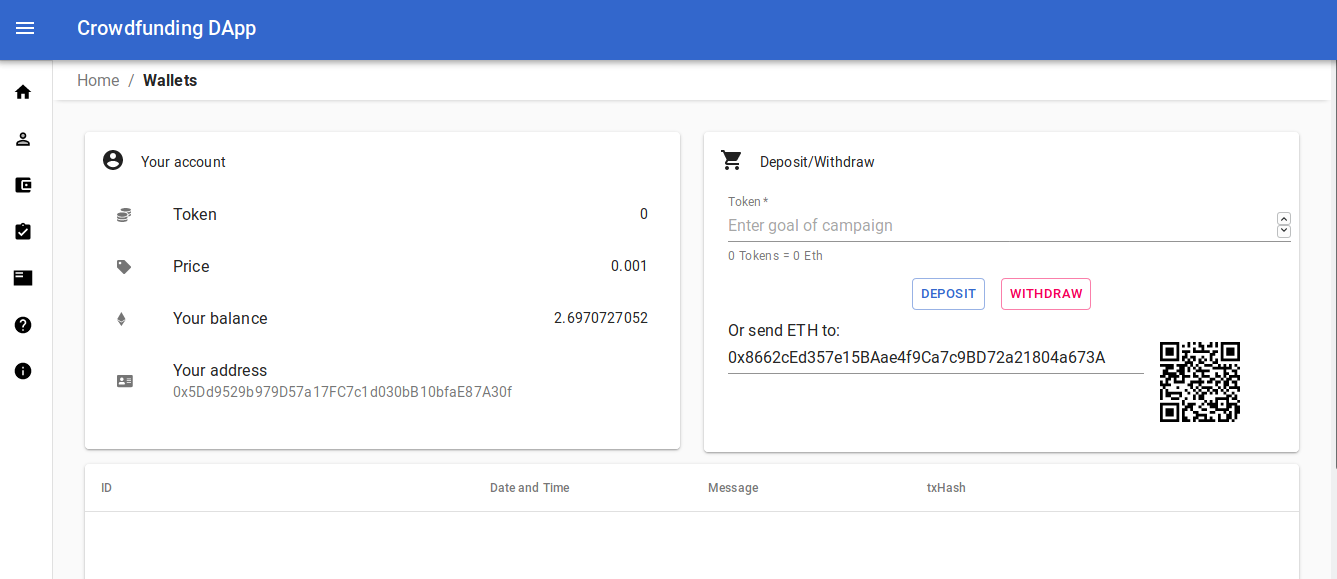
\includegraphics[scale=0.32]{ui-wallet}
\caption{Màn hình giao diện trang nộp tiền và rút tiền}
\end{center}
\end{figure}

Nhân viên vận hành tiến hành thêm vào các nhân viên xác minh, ảnh chụp giao diện người dùng của trang thêm nhân viên xác minh ở hình \ref{fig:ui-add-verifier}.

\begin{figure}[ht!]
\begin{center}
\label{fig:ui-add-verifier}
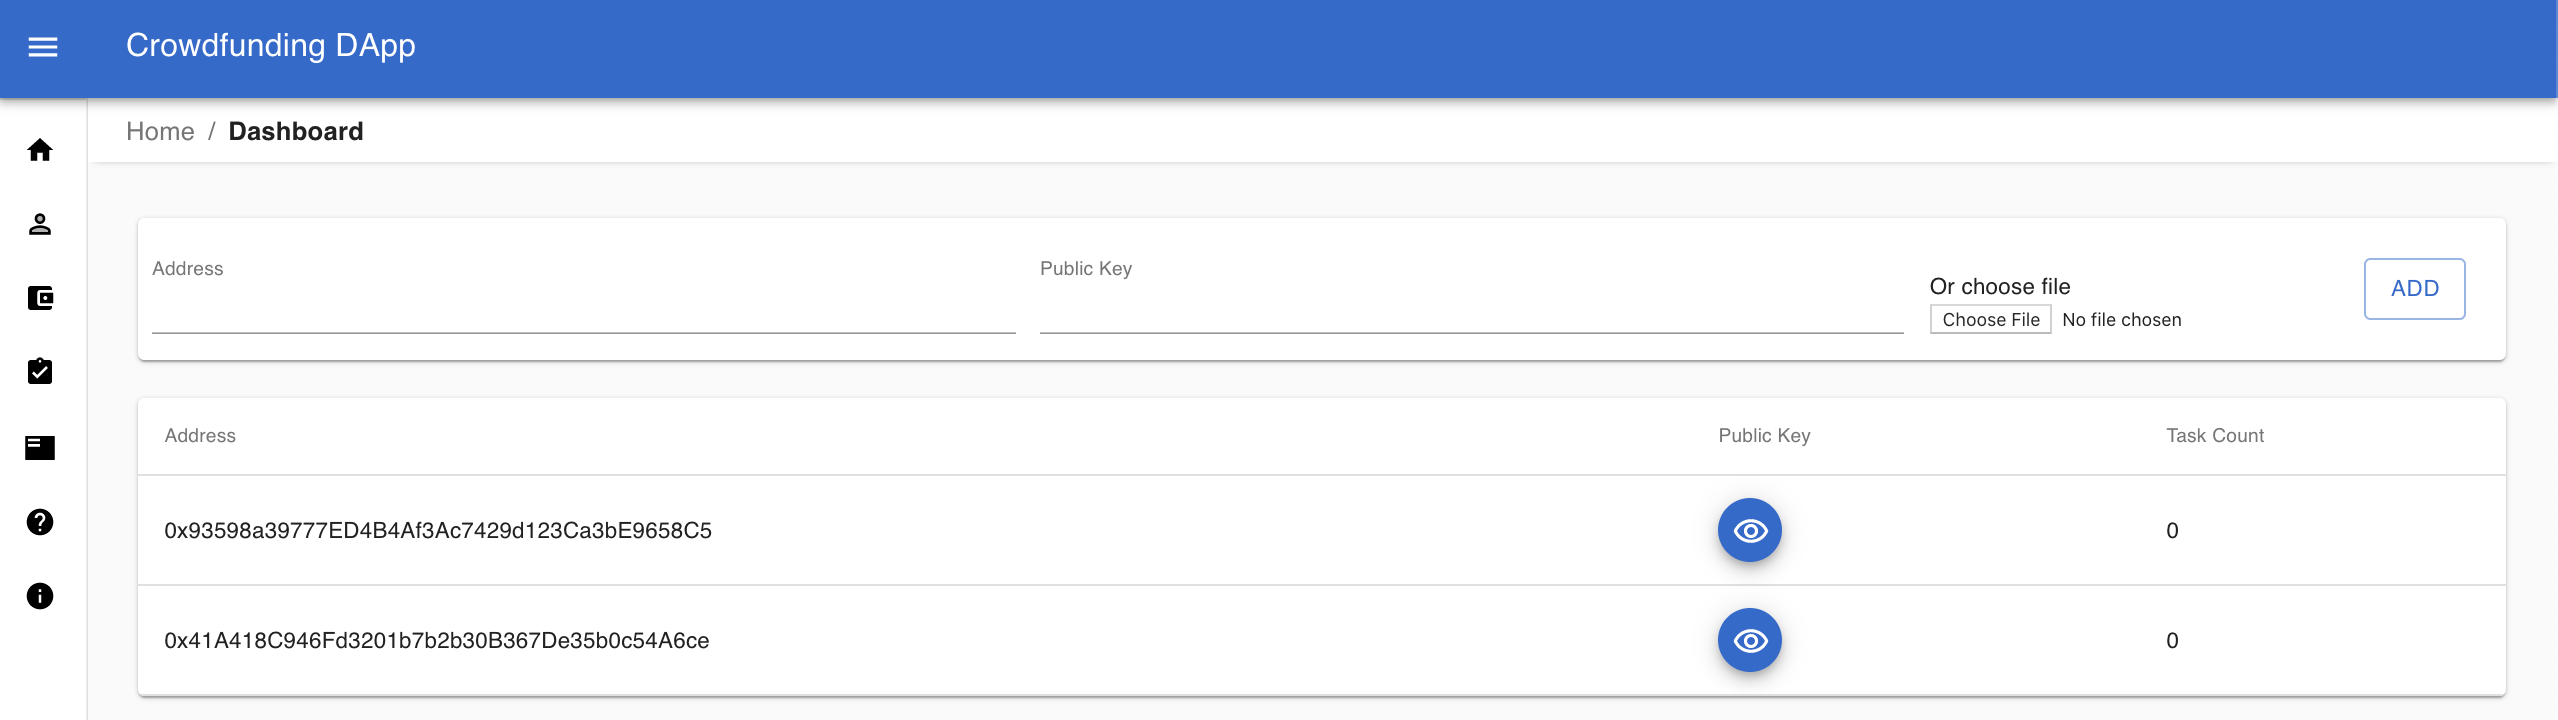
\includegraphics[scale=0.34]{ui-add-verifier}
\caption{Màn hình giao diện trang thêm nhân viên xác minh}
\end{center}
\end{figure}

Tiếp theo, người tạo chiến dịch tiến hành đăng kí hồ sơ định danh, giao diện trang đăng kí thông tin định danh dành cho người tạo chiến dịch được thể hiện ở hình \ref{fig:ui-register-identity}. Người tạo chiến dịch sẽ nhập các thông tin cần thiết theo mẫu, sau đó nhấn vào nút \textbf{``Submit''}.

\begin{figure}[ht!]
\begin{center}
\label{fig:ui-register-identity}
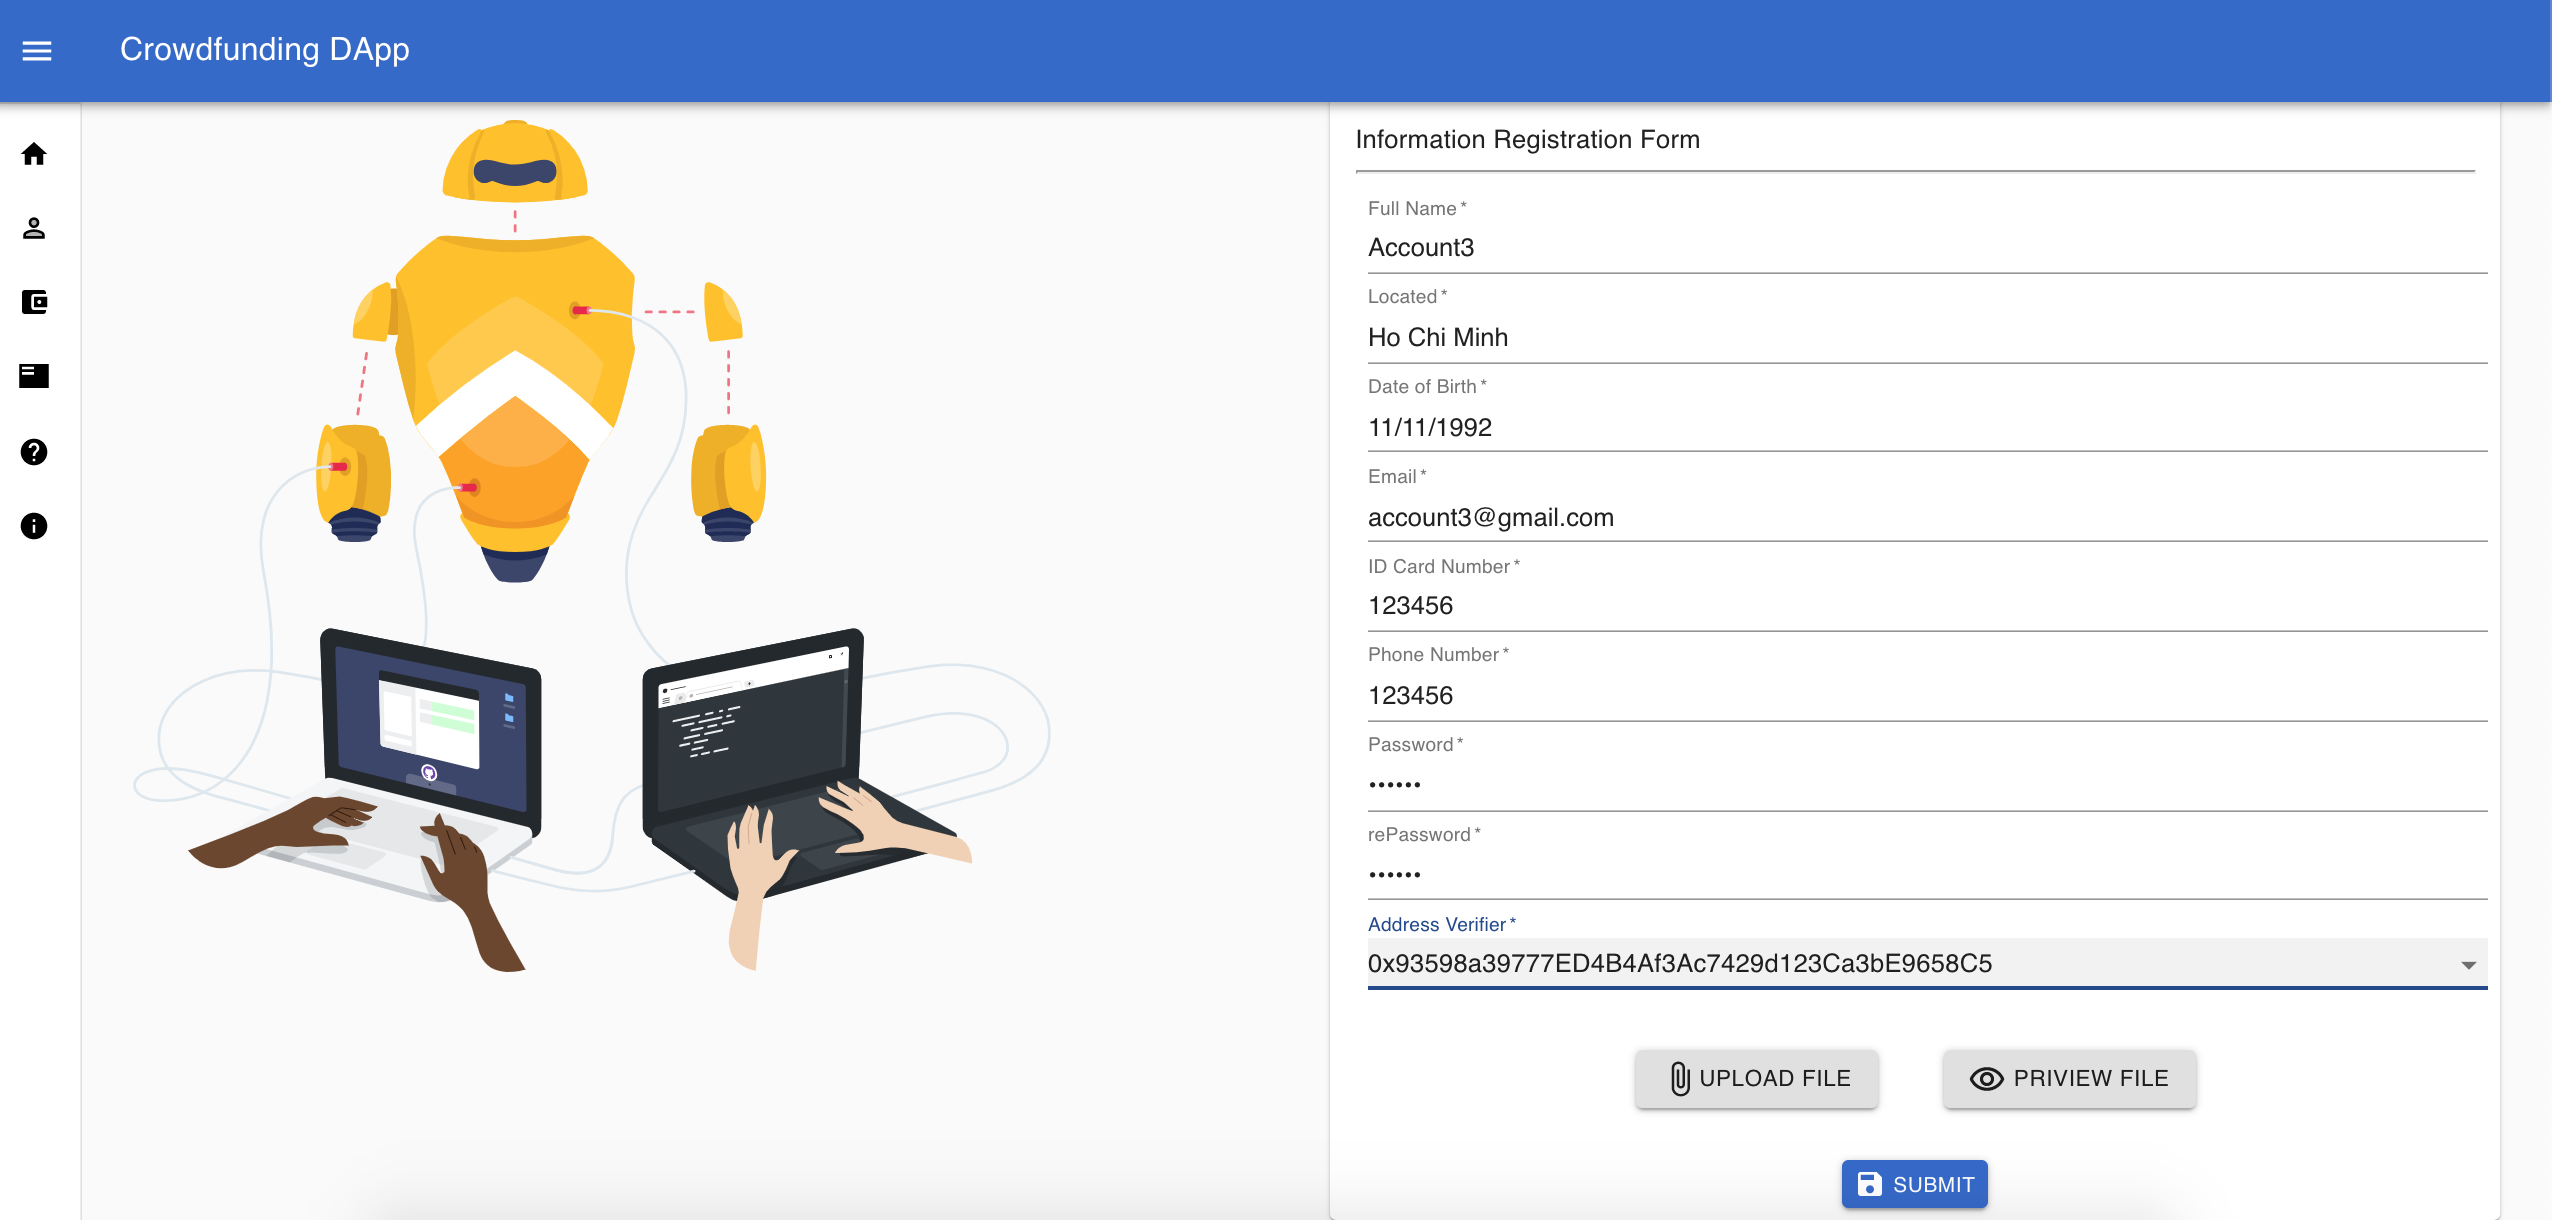
\includegraphics[scale=0.33]{ui-register-identity}
\caption{Màn hình giao diện trang đăng kí định danh}
\end{center}
\end{figure}

Sau đó, một hộp thoại sẽ xuất hiện để xác nhận lại các điều khoản, nếu chấp nhận các điều khoản thì sẽ tiến hành tạo \gls{transaction}. Sau đó transaction được kí bởi Metamask, một hộp thoại khác được hiển thị để xác nhận phía Metamask như ở hình \ref{fig:ui-metamask-confirm-1}.


\begin{figure}[ht!]
\begin{center}
\label{fig:ui-metamask-confirm-1}
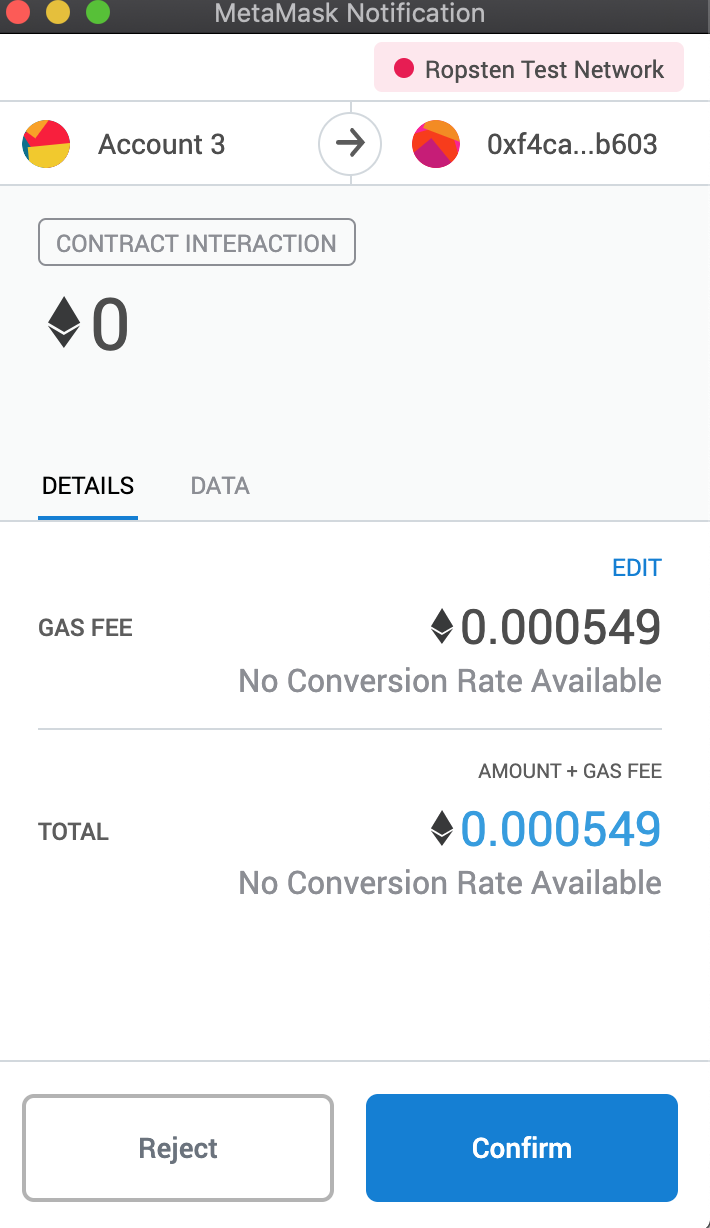
\includegraphics[scale=0.5]{ui-metamask-confirm-1}
\caption{Màn hình hộp thoại xác nhận kí transaction trên Metamask}
\end{center}
\end{figure}

Transaction sau khi được kí sẽ được gửi đến mạng blockchain, có thể xem chi tiết transaction trên Etherscan\footnote{https://etherscan.io}, hình \ref{fig:ui-transaction-detail} là ảnh chụp chi tiết transacion.

\begin{figure}[ht!]
\begin{center}
\label{fig:ui-transaction-detail}
\fbox{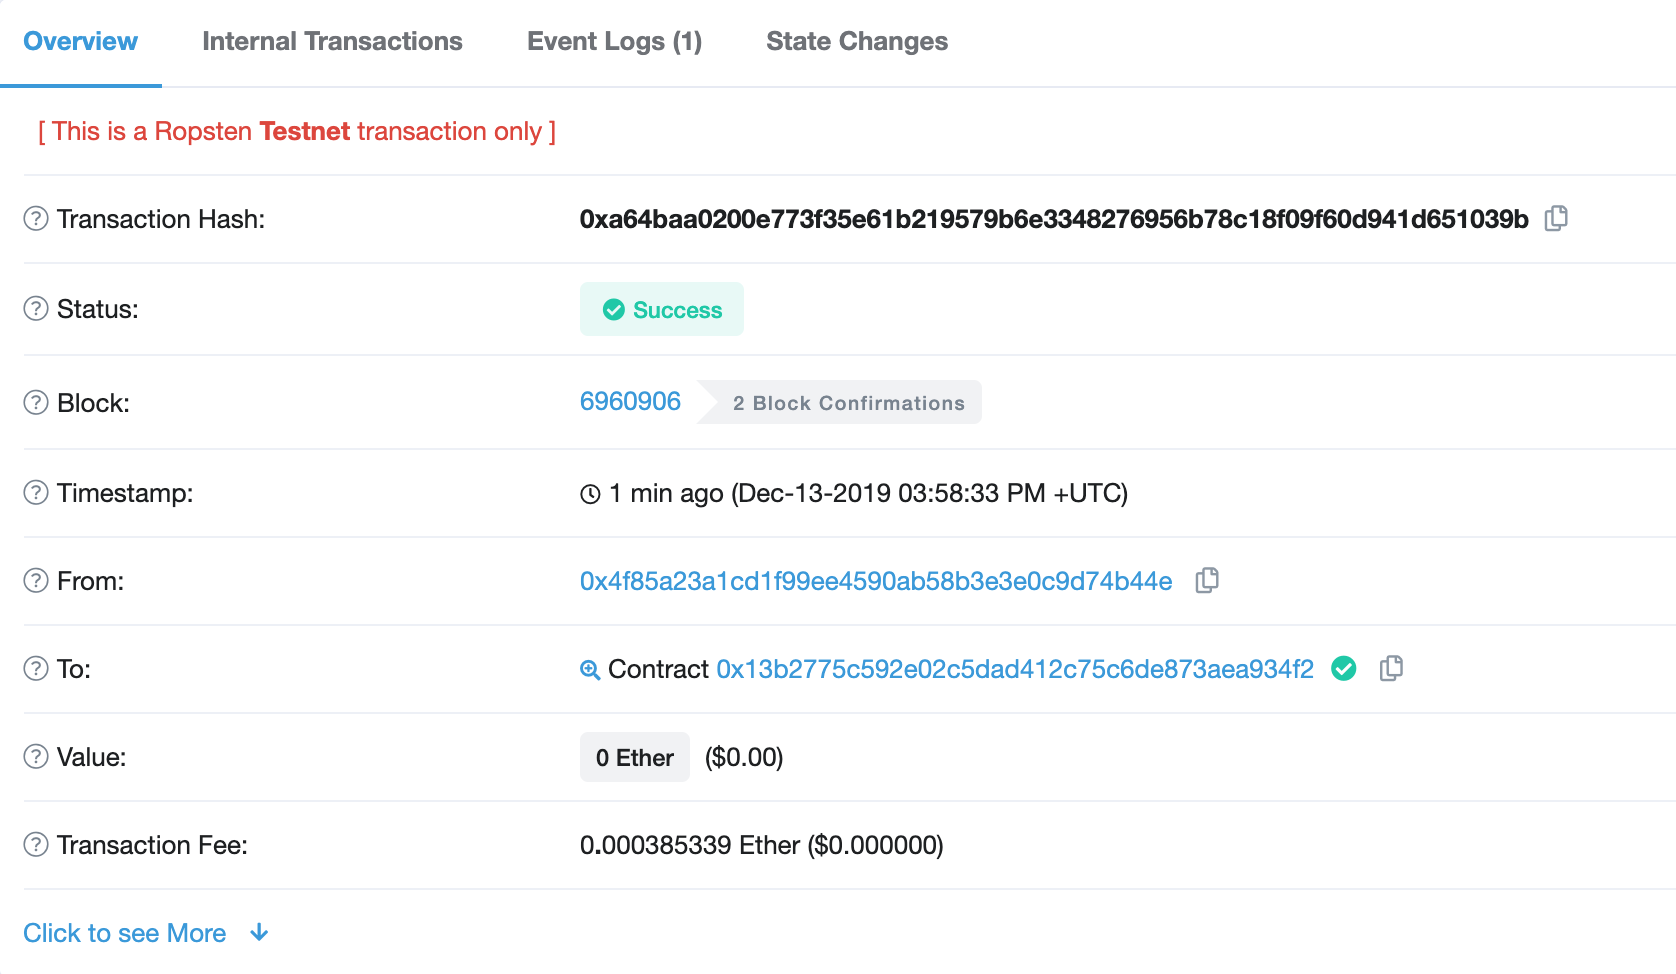
\includegraphics[scale=0.5]{ui-transaction-detail}}
\caption{Ảnh chụp chi tiết transaction trên etherscan}
\end{center}
\end{figure}

Tiếp theo, nhân viên xác minh tiến hành kiểm tra các danh sách các hồ sơ định danh, màn hình hiển thị danh sách người dùng đã đăng kí hồ sơ định danh được thể hiện ở hình \ref{fig:ui-list-user}.

\begin{figure}[ht!]
\begin{center}
\label{fig:ui-list-user}
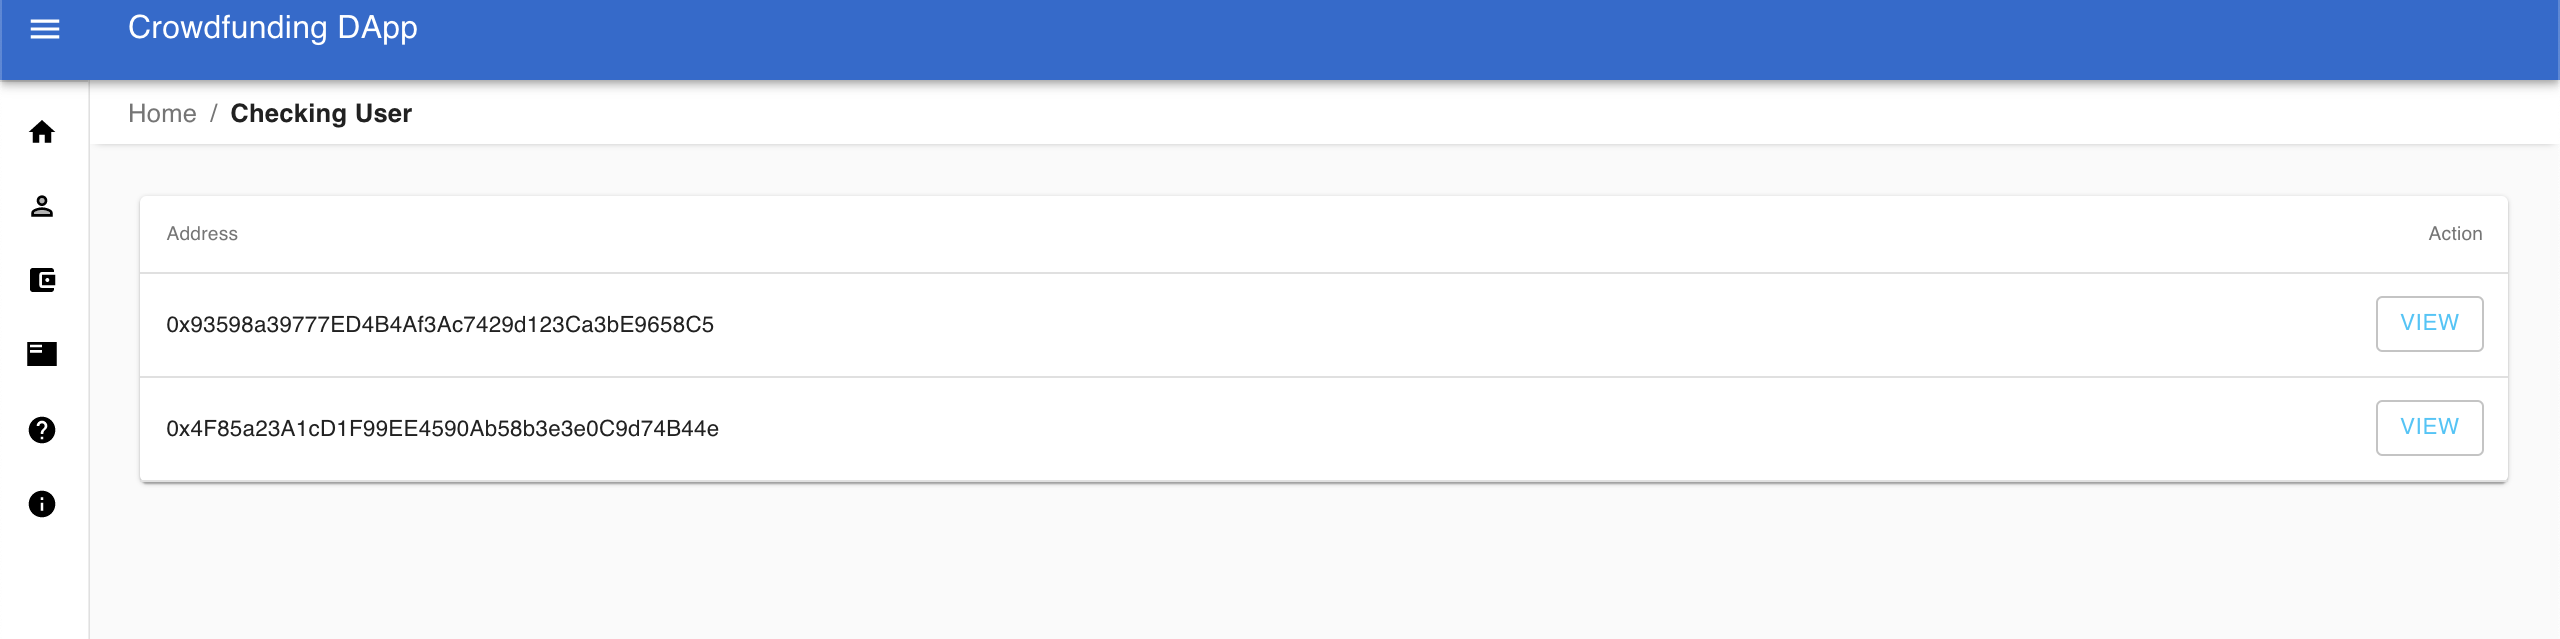
\includegraphics[scale=0.34]{ui-list-user}
\caption{Giao diện trang hiển thị danh sách hồ sơ định danh}
\end{center}
\end{figure}

Ứng với từng địa chỉ, ấn nút \textbf{``VIEW''} để xem chi tiết thông tin ở từng hồ sơ. Sau đó, một hộp thoại hiện lên chứa các thông tin như ở hình \ref{fig:ui-identity-view}. Để xem thông tin bí mật chia sẻ từ người tạo lập hồ sơ, nhân viên xác minh cần nhập khóa bí mật của mình. Sau khi xem xét tất cả thông tin cần thiết, nhân viên xác minh có thể chấp nhận hồ sơ đó bằng cách nhấn vào nút \textbf{``ALLOW''} hoặc từ chối với nút \textbf{``REJECT''}. Hồ sơ định danh được chấp nhận thì người tạo chiến dịch mới được quyền tạo chiến dịch gây quỹ.

\begin{figure}[ht!]
\begin{center}
\label{fig:ui-identity-view}
\fbox{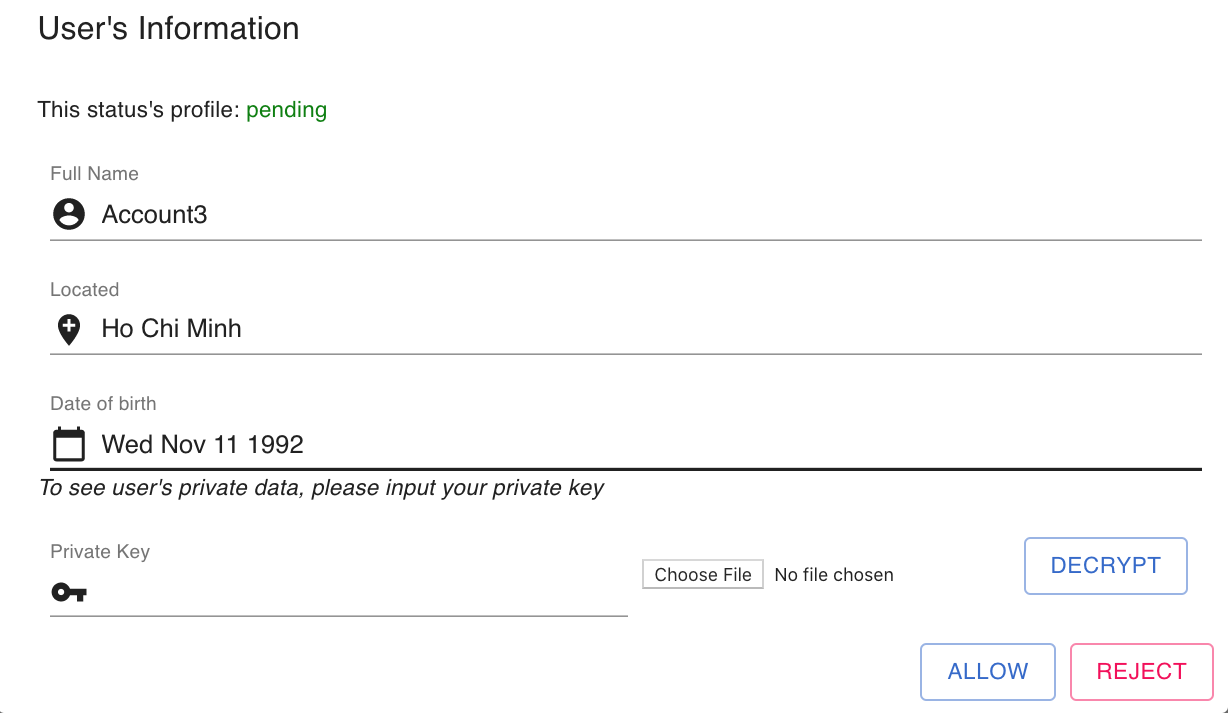
\includegraphics[scale=0.7]{ui-identity-view}}
\caption{Màn hình hiển thị thông tin định danh người dùng}
\end{center}
\end{figure}

Nếu hồ sơ định danh được xét duyệt, người tạo chiến dịch có thể đăng kí chiến dịch gây quỹ. Giao diện người dùng của trang đăng kí chiến dịch như ở hình \ref{fig:ui-create-campaign}.

\begin{figure}[ht!]
\begin{center}
\label{fig:ui-create-campaign}
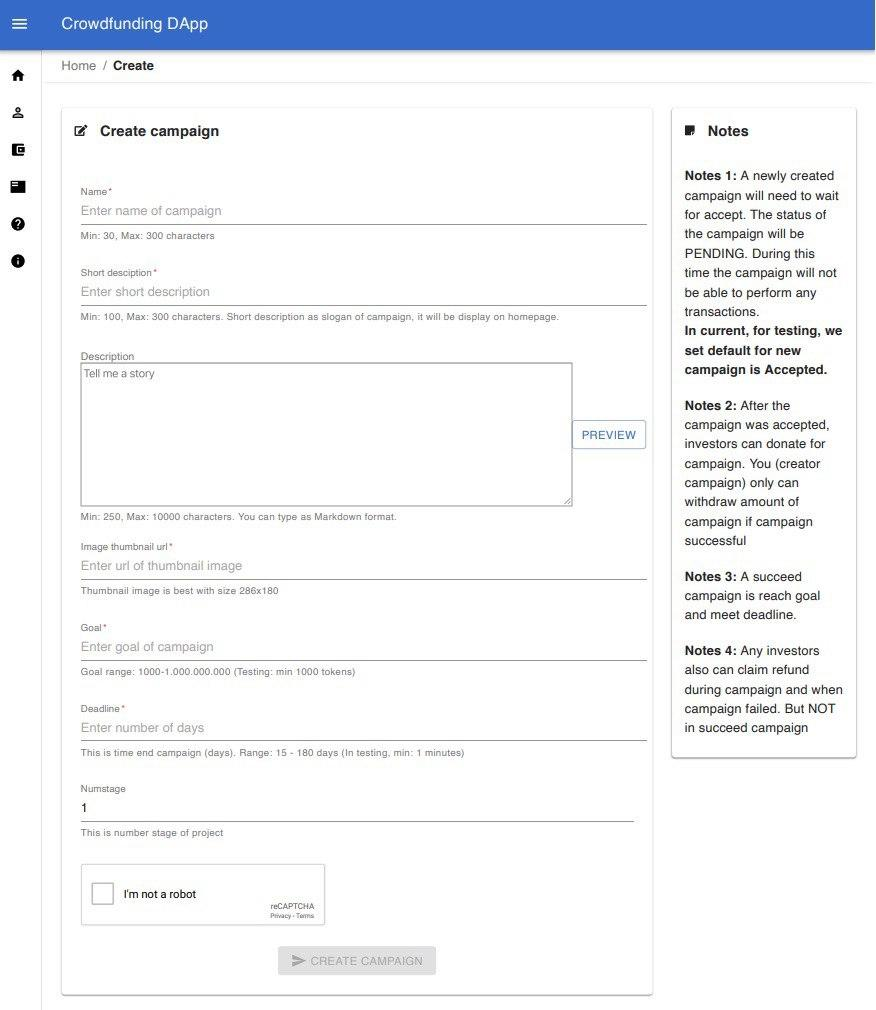
\includegraphics[scale=0.5]{ui-create-campaign.jpg}
\caption{Giao diện trang đăng kí chiến dịch gây quỹ}
\end{center}
\end{figure}

Sau khi người tạo chiến dịch gửi transaction đi thành công thì chiến dịch đó tạm thời được gán trạng thái là đang chờ xét duyệt. Nhân viên xác minh sẽ tiến hành đọc thông tin chiến dịch và xét duyệt chiến dịch đó. Màn hình hiển thị thông tin chiến dịch chờ xét từ nhân viên xác minh được thể hiện ở hình \ref{fig:ui-campaign-pending}, lưu ý trang này chỉ dành cho nhân viên xác minh.

\begin{figure}[ht!]
\begin{center}
\label{fig:ui-campaign-pending}
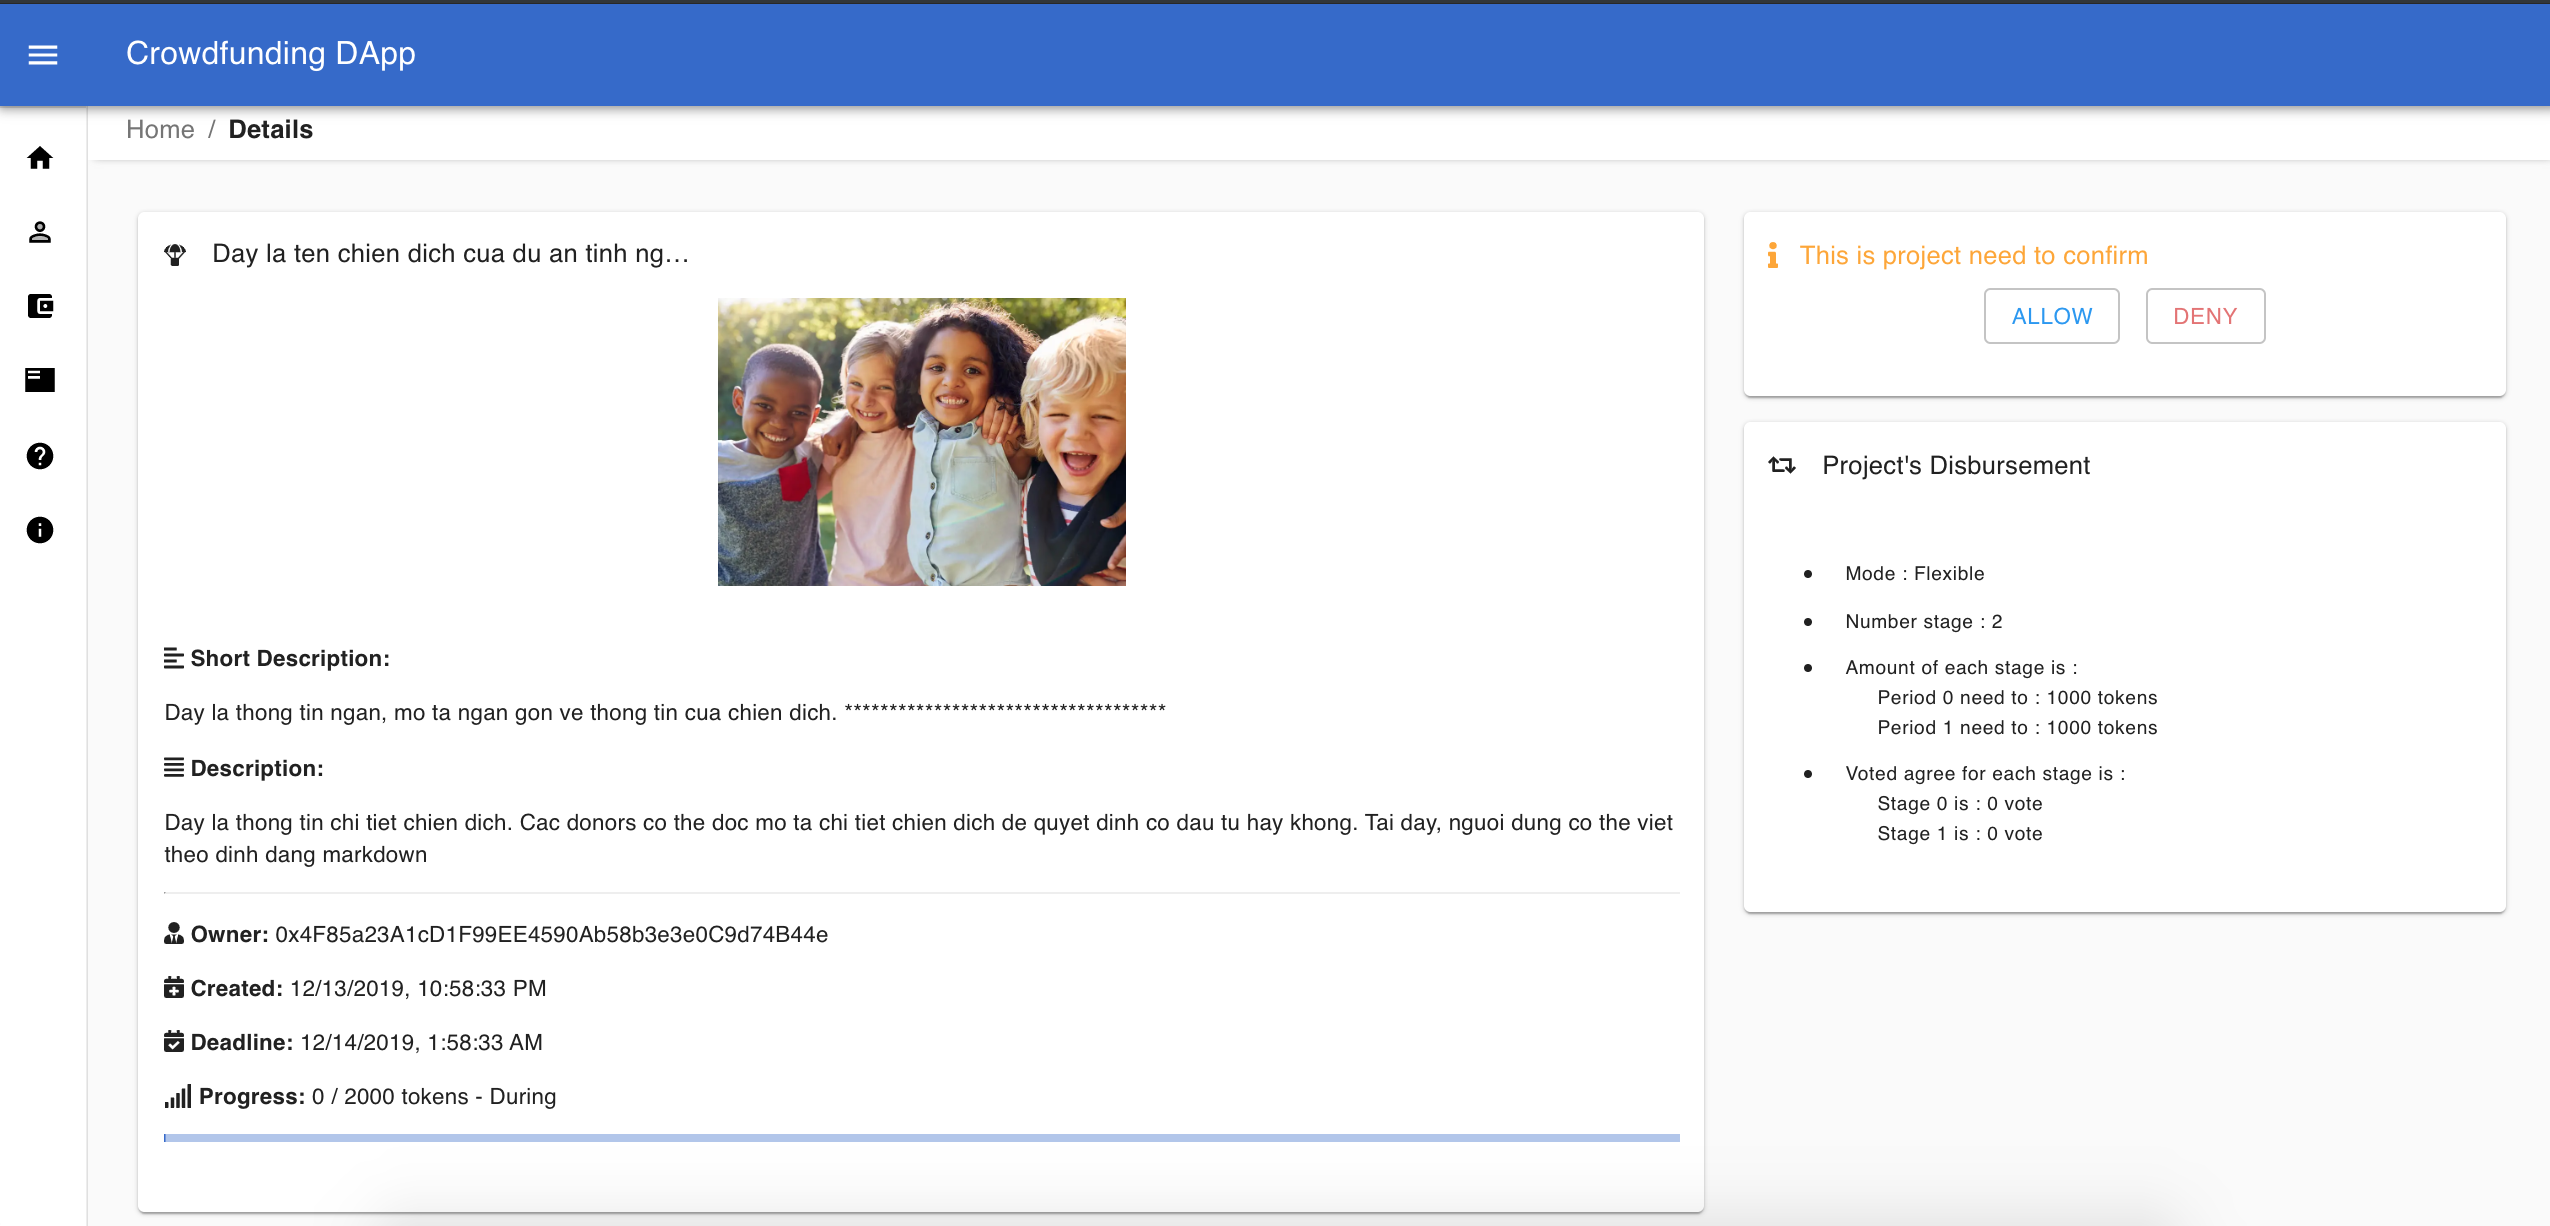
\includegraphics[scale=0.34]{ui-campaign-pending}
\caption{Giao diện người dùng khi xem thông tin chiến dịch đang chờ xét duyệt}
\end{center}
\end{figure}

Chỉ có những chiến dịch nào được xét duyệt cho đồng ý đóng góp thì mới được xuất hiện trong danh sách chiến dịch cho người đóng góp thấy. Hình \ref{fig:ui-list-campaign} là ảnh chụp giao diện danh sách các chiến dịch đã được xác minh để người đóng góp có thể nhìn thấy được. Tại danh sách các chiến dịch, người đóng góp có thể thấy được các thông tin tổng quát của chiến dịch như thời gian bắt đầu, thời gian kết thúc chiến dịch, trạng thái của chiến dịch, \ldots.

\begin{figure}[ht!]
\begin{center}
\label{fig:ui-list-campaign}
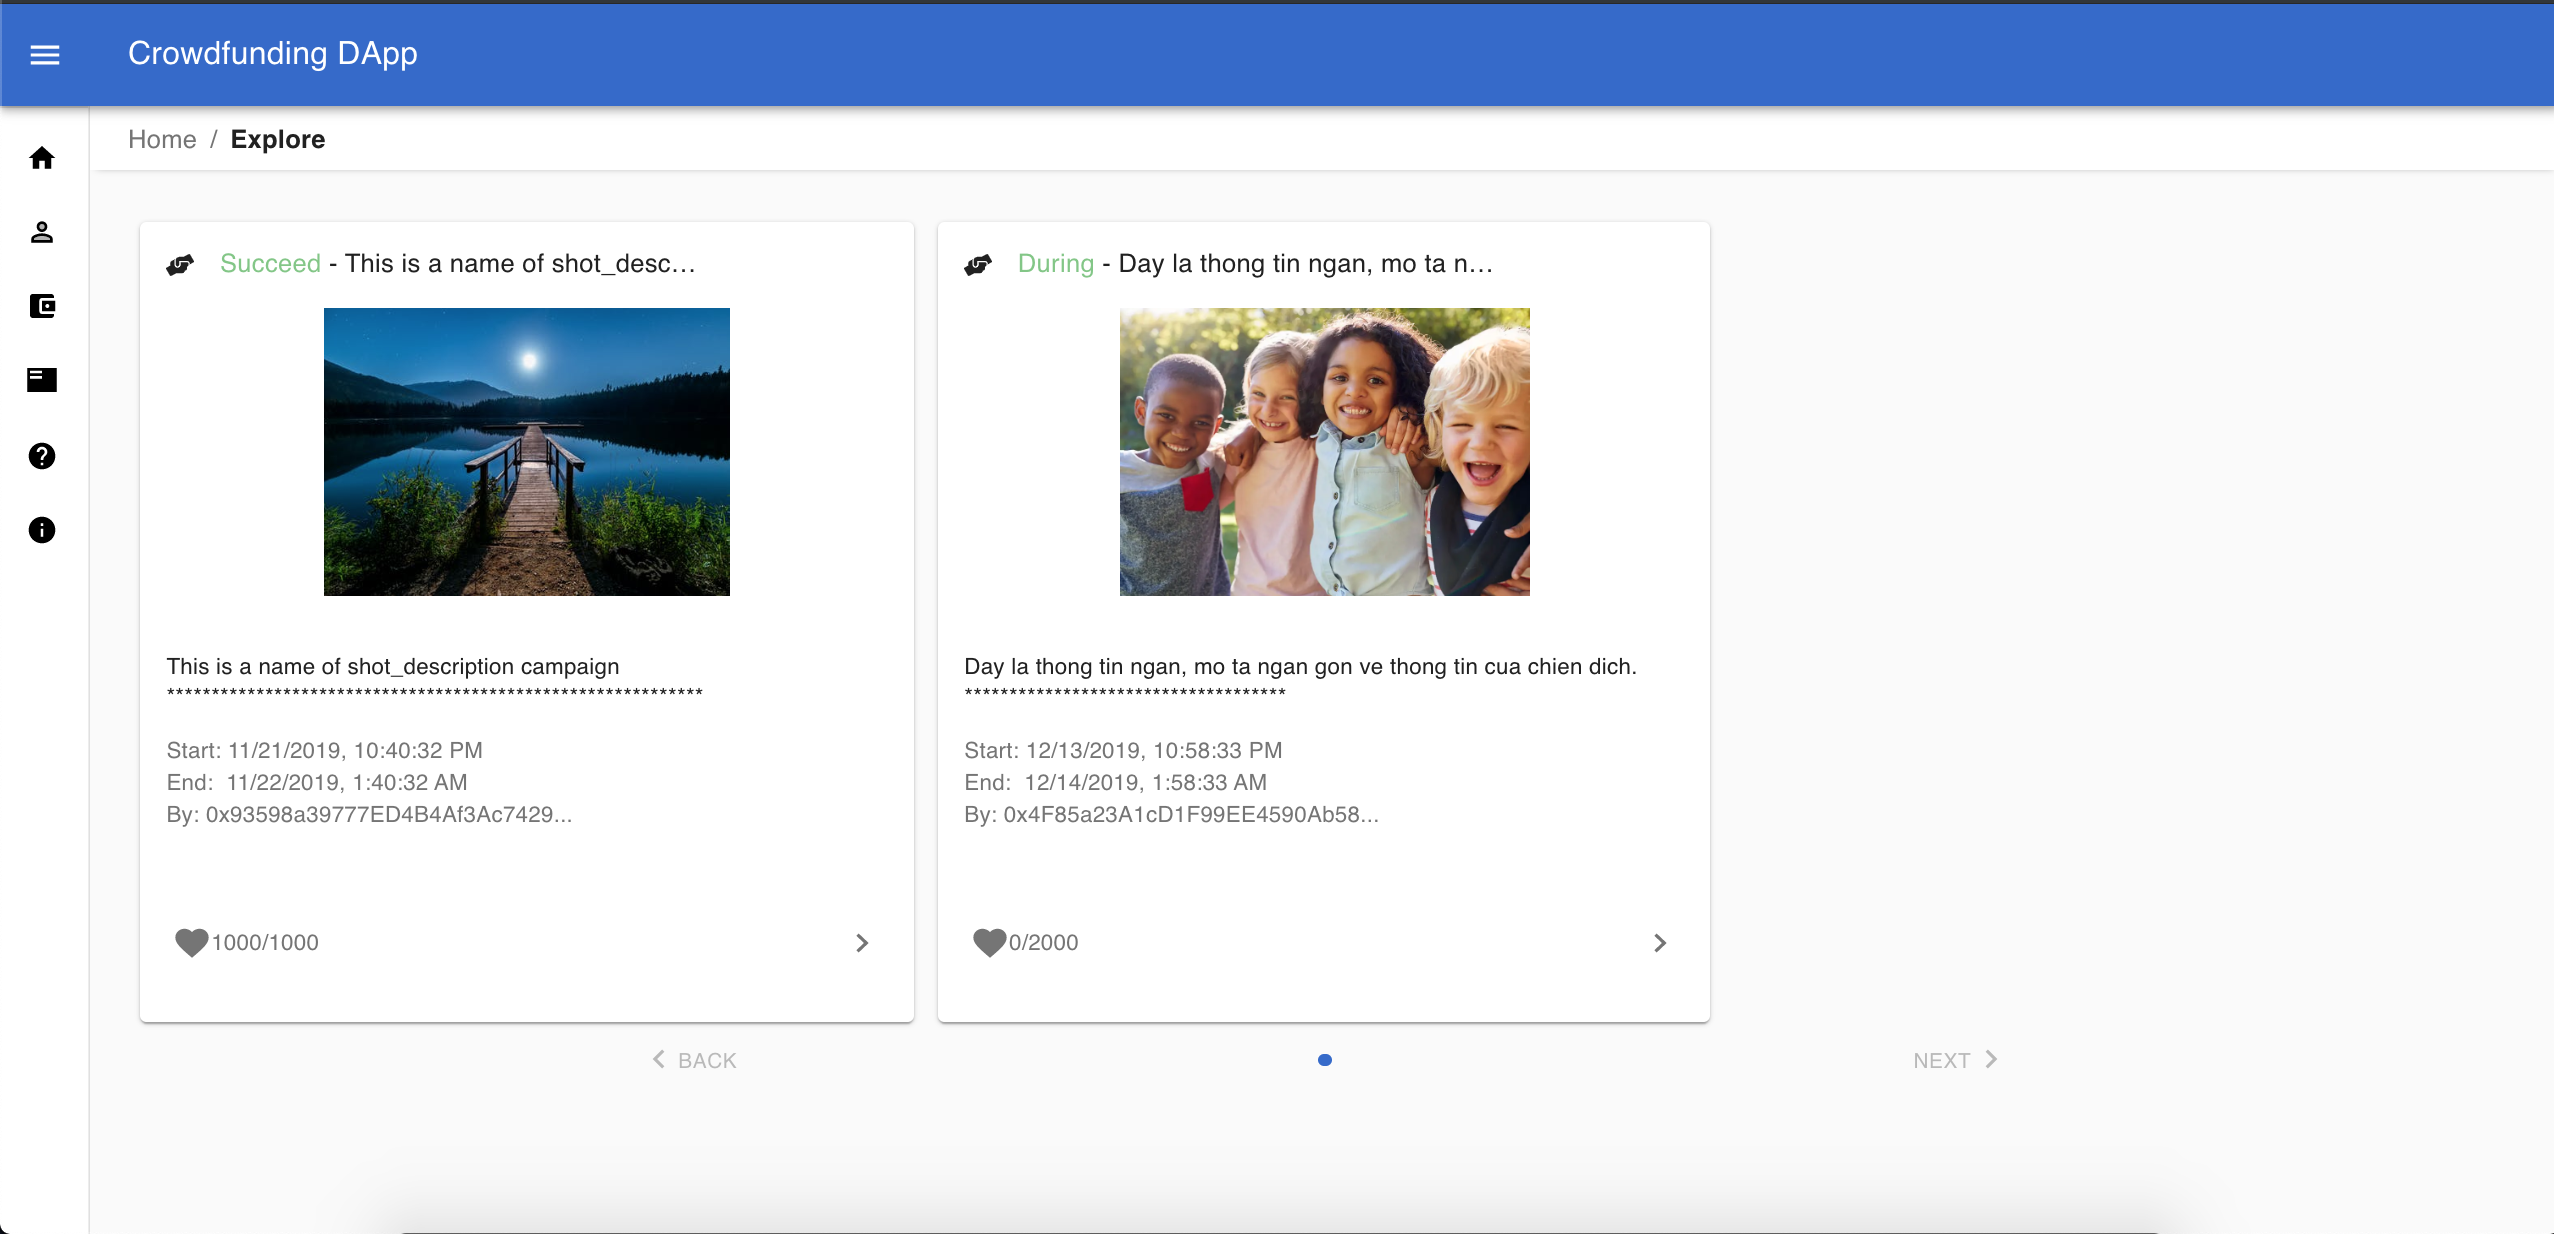
\includegraphics[scale=0.34]{ui-list-campaign}
\caption{Giao diện của trang danh sách các chiến dịch}
\end{center}
\end{figure}

Để xem thông tin chi tiết của chiến dịch, người đóng góp có thể ấn chọn chiến dịch đó và sau đó là trang thông tin chi tiết chiến dịch như ở hình \ref{fig:ui-detail-campaign}.

\begin{figure}[ht!]
\begin{center}
\label{fig:ui-detail-campaign}
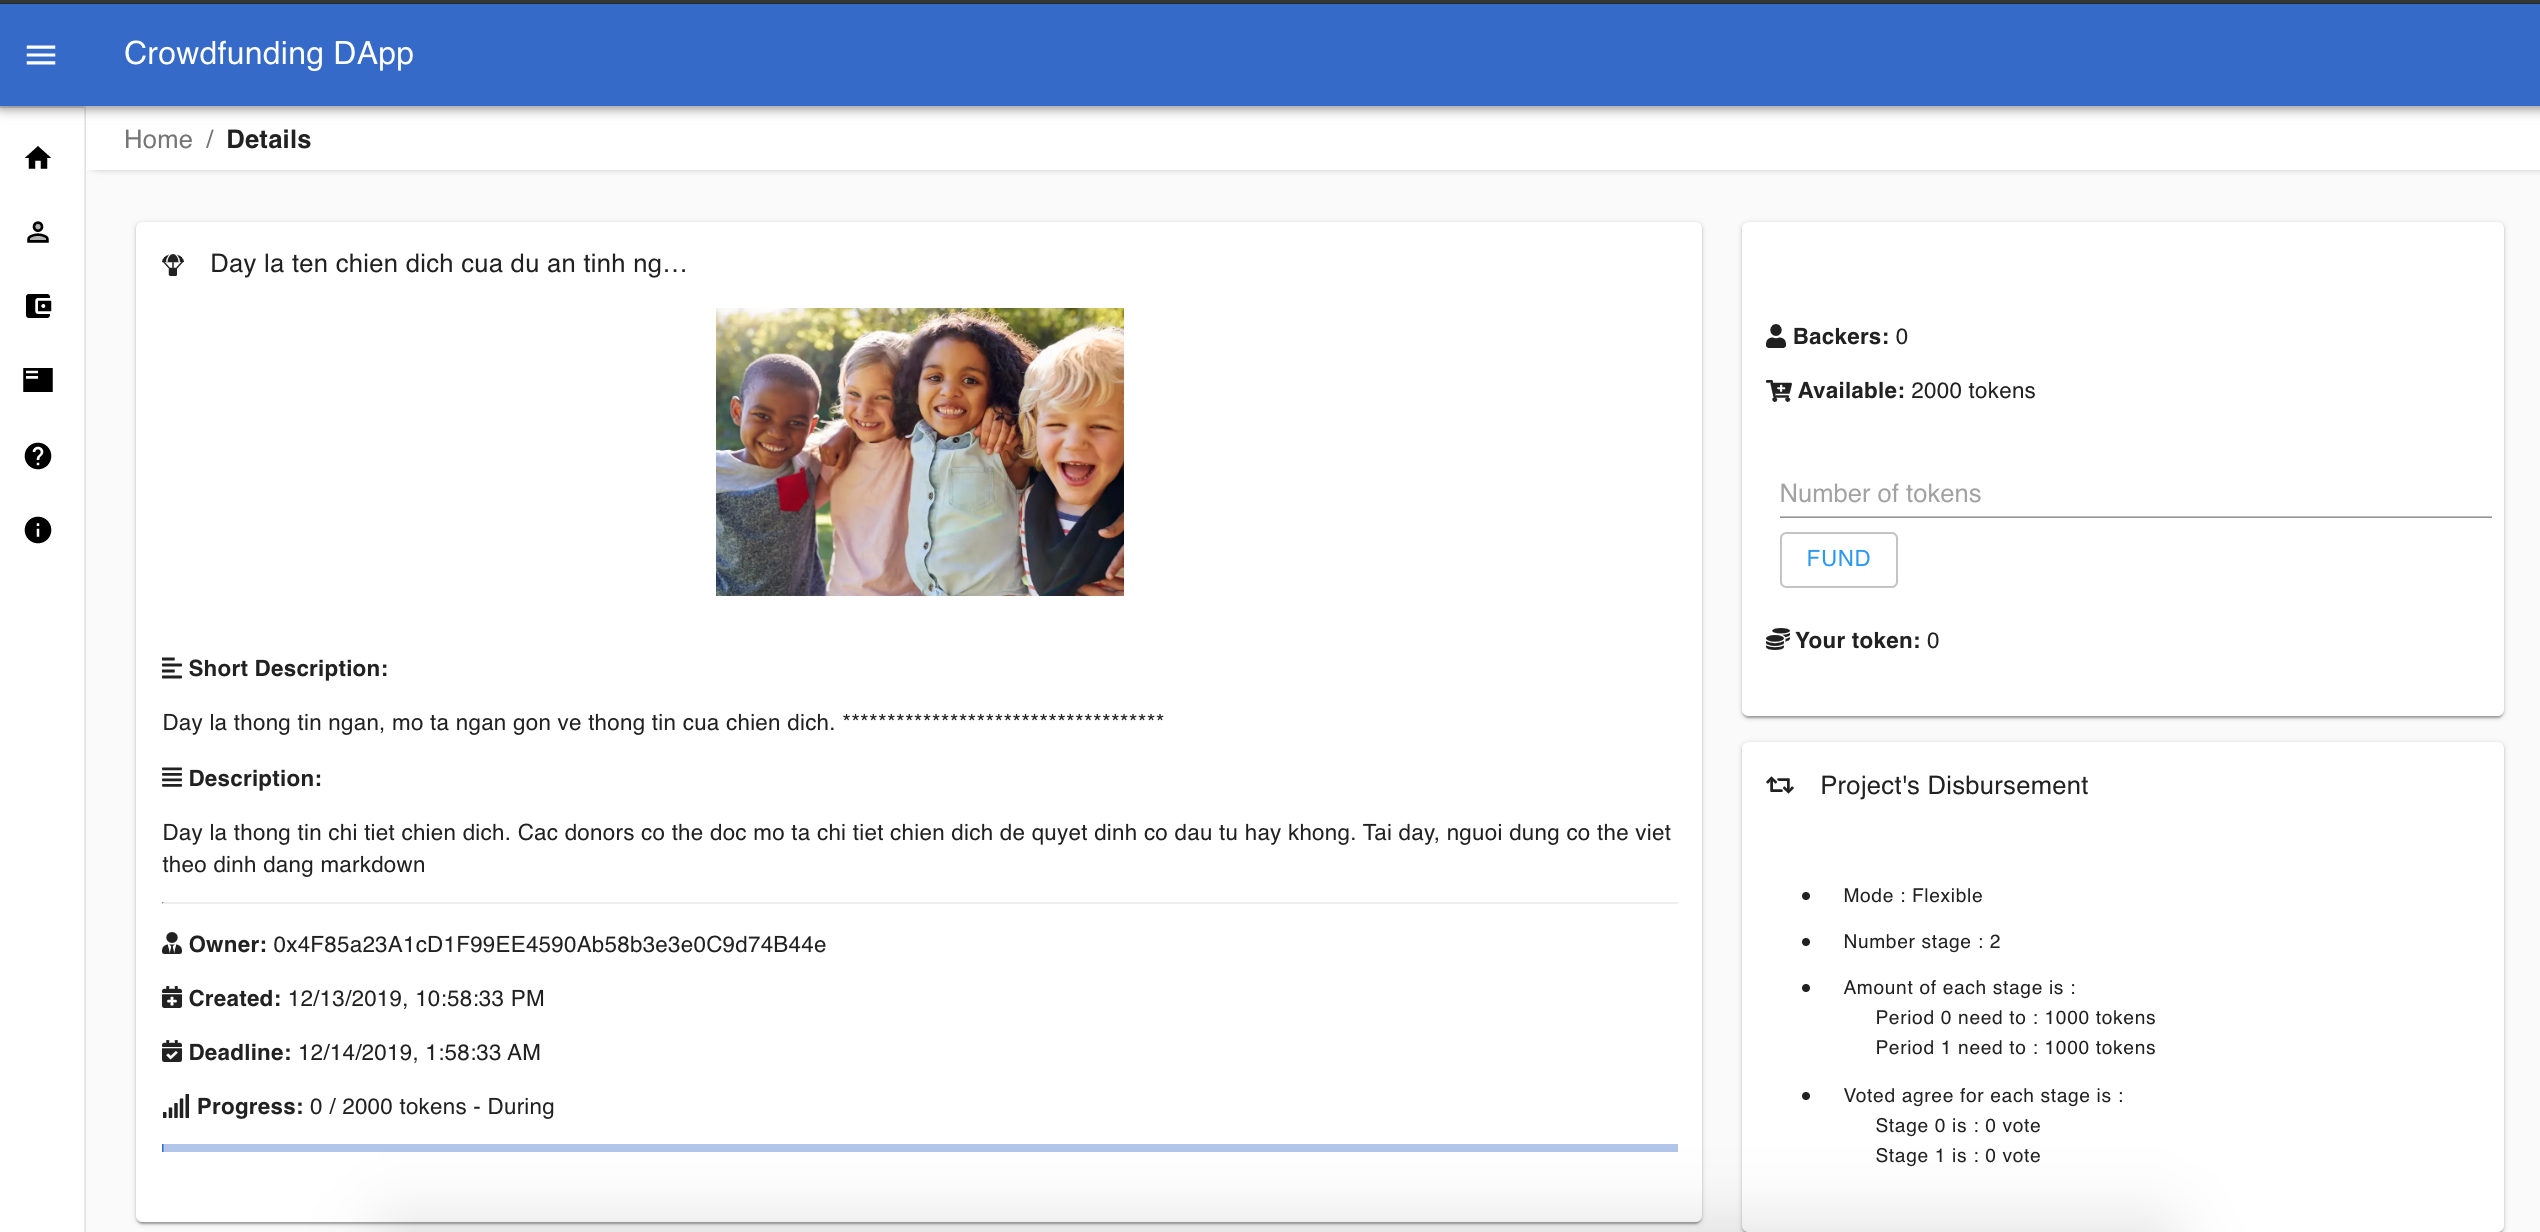
\includegraphics[scale=0.34]{ui-detail-campaign}
\caption{Giao diện của trang chi tiết thông tin chiến dịch}
\end{center}
\end{figure}

\section{Đánh giá hệ thống đã hiện thực}
\subsection{Kiểm tra các quy trình trong hệ thống}
\subsubsection{Mục tiêu}
Kiểm tra các quy trình trong hệ thống nhằm mục tiêu sau:

\begin{itemize}
\item Xác định đầu ra các hàm trong hợp đồng thông minh có trả về kết quả đúng như mong đợi với đầu vào cho trước hay không.
\item Việc thực hiện kiểm tra các hàm tuần tự như quy trình hoạt động thực tế của hệ thống.
\item Phát hiện các lỗi ở mức đơn vị nhỏ nhất trong hệ thống.
\end{itemize}
\subsubsection{Phương pháp thực hiện}
Nhóm tác giả tiến hành kiểm thử đơn vị (unit testing) với các hàm trong hệ thống theo hai kịch bản. Bao gồm:

\begin{itemize}
\item \textbf{Kịch bản 1:} kiểm thử quy trình với chiến dịch một giai đoạn.
\item \textbf{Kịch bản 2:} kiểm thử quy trình với chiến dịch nhiều giai đoạn.
\end{itemize}

Kịch bản 1 được nhóm tác giả soạn như sau:

\begin{enumerate}[label=(\arabic*)]
\item Nhân viên vận hành tiến hành biên dịch và triển khai các hợp đồng thông minh lên mạng blockchain. Kiểm tra kết quả: địa chỉ các hợp đồng thông minh đã có trên mạng blockchain hay chưa?
\item Người đóng góp gọi hàm \textit{deposit} để nộp tiền vào hệ thống. Kiểm tra kết quả: chênh lệch số dư trước và sau khi gọi hàm có bằng số tiền đã nộp?
\item Người vận hành gọi hàm \textit{addVerify} để thêm danh sách xác nhân viên xác minh. Kiểm tra kết quả: địa chỉ có trong danh sách địa chỉ nhân viên xác minh?
\item Người tạo chiến dịch gọi hàm \textit{registerIdentity} để đăng kí hồ sơ định danh. Kiểm tra kết quả: lấy thông tin hồ sơ định danh đã lưu đối chiếu với đầu vào trước đó đã nhập, hai thông tin có giống nhau?
\item Nhân viên xác minh gọi hàm \textit{verify} để xác minh cho một hồ sơ định danh. Kiểm tra kết quả: trạng thái của hồ sơ định danh đã được xác minh hay chưa?
\item Người tạo chiến dịch gọi hàm \textit{createCampaign} để tạo chiến dịch thứ nhất. Kiểm tra kết quả: đối chiếu thông tin chiến dịch đã lưu với đầu vào đã nhập có khớp nhau?
\item Nhân viên xác minh gọi hàm \textit{verifyCampaign} để xác minh cho chiến dịch, cho phép chiến dịch được nhận đóng góp từ người dùng. Kiểm tra kết quả: trạng thái chiến dịch có được xác minh hay chưa?
\item Người đóng góp gọi hàm \textit{donate} để đóng góp tiền cho chiến dịch, số tiền đóng góp đúng bằng mục tiêu của chiến dịch. Kiểm tra kết quả: chênh lệch số dư trước và sau khi đóng góp có bằng với số tiền đã đóng góp?
\item Người tạo chiến dịch tiến hành gọi hàm \textit{endCampaign} để gọi lệnh giải ngân từ chiến dịch khi kết thúc thời gian chiến dịch gây quỹ. Kiểm tra kết quả: chênh lệch số dư (tokens) của người tạo chiến dịch trước và sau khi gọi lệnh giải ngân đúng bằng số tiền đã đóng góp hay không?
\item Người tạo chiến dịch gọi hàm \textit{createCampaign} để tạo chiến dịch thứ hai. Kiểm tra kết quả: đối chiếu thông tin chiến dịch đã lưu với đầu vào đã nhập có khớp nhau?
\item Nhân viên xác minh gọi hàm \textit{verifyCampaign} để xác minh cho chiến dịch, cho phép chiến dịch được nhận đóng góp từ người dùng. Kiểm tra kết quả: trạng thái chiến dịch có được xác minh hay chưa?
\item Người đóng góp gọi hàm \textit{donate} để đóng góp tiền cho chiến dịch, số tiền đóng góp không đạt được mục tiêu gây quỹ. Kiểm tra kết quả: chênh lệch số dư trước và sau khi đóng góp có bằng với số tiền đã đóng góp?
\item Sau khi kết thúc thời gian gây quỹ, người đóng góp tiến hành kiểm tra số dư có đúng bằng số tiền đã đúng bằng số tiền đã đóng góp hay không?
\end{enumerate}

Kịch bản 2 như sau:

\begin{enumerate}[label=(\arabic*)]
\item Nhân viên vận hành tiến hành biên dịch và triển khai các hợp đồng thông minh lên mạng blockchain. Kiểm tra kết quả: địa chỉ các hợp đồng thông minh đã có trên mạng blockchain hay chưa?
\item Người đóng góp gọi hàm \textit{deposit} để nộp tiền vào hệ thống, số lượng tài khoản người đóng góp là 5 và mỗi tài khoản sẽ có 1500 tokens dùng cho đóng góp chiến dịch. Kiểm tra kết quả: chênh lệch số dư trước và sau khi gọi hàm có bằng số tiền đã nộp?
\item Người vận hành gọi hàm \textit{addVerify} để thêm danh sách xác nhân viên xác minh. Kiểm tra kết quả: địa chỉ có trong danh sách địa chỉ nhân viên xác minh?
\item Người tạo chiến dịch gọi hàm \textit{registerIdentity} để đăng kí hồ sơ định danh. Kiểm tra kết quả: lấy thông tin hồ sơ định danh đã lưu đối chiếu với đầu vào trước đó đã nhập, hai thông tin có giống nhau?
\item Nhân viên xác minh gọi hàm \textit{verify} để xác minh cho một hồ sơ định danh. Kiểm tra kết quả: trạng thái của hồ sơ định danh đã được xác minh hay chưa?
\item Người tạo chiến dịch gọi hàm \textit{createCampaign} để tạo chiến dịch thứ nhất, chiến dịch thứ nhất có 3 giai đoạn giải ngân. Kiểm tra kết quả: đối chiếu thông tin chiến dịch đã lưu với đầu vào đã nhập có khớp nhau?
\item Nhân viên xác minh gọi hàm \textit{verifyCampaign} để xác minh cho chiến dịch, cho phép chiến dịch được nhận đóng góp từ người dùng. Kiểm tra kết quả: trạng thái chiến dịch có được xác minh hay chưa?
\item Người đóng góp gọi hàm \textit{donate} để đóng góp tiền cho chiến dịch, số tiền đóng góp đúng bằng mục tiêu của chiến dịch. Kiểm tra kết quả: chênh lệch số dư trước và sau khi đóng góp có bằng với số tiền đã đóng góp?
\item Người tạo chiến dịch tiến hành gọi hàm \textit{endCampaign} để gọi lệnh giải ngân giai đoạn đầu tiên từ chiến dịch khi kết thúc thời gian chiến dịch gây quỹ. Kiểm tra kết quả: chênh lệch số dư (tokens) của người tạo chiến dịch trước và sau khi gọi lệnh giải ngân đúng bằng số tiền được giải ngân ở giai đoạn đầu tiên hay không?
\item Người đóng góp tiến hành gọi hàm \textit{vote} để bình chọn cho giai đoạn thứ hai trở đi. Kiểm tra kết quả: danh sách đã bình chọn cho giai đoạn giải ngân của chiến dịch có địa chỉ của người đóng góp hay không?
\item Người tạo chiến dịch tiến hành gọi hàm \textit{endCampaign} lần nữa để gọi lệnh giải ngân giai đoạn tiếp theo. Kiểm tra kết quả: chênh lệch số dư (tokens) của người tạo chiến dịch trước và sau khi gọi lệnh giải ngân đúng bằng số tiền được giải ngân ở giai đoạn đó hay không?
\end{enumerate}

Với kịch bản 2, nhóm tác giả tiến hành tạo ra nhiều chiến dịch khác nhau, sau đó người đóng góp tiến hành biểu quyết với tỉ lệ đồng ý khác nhau. Kịch bản được nhóm tác giả hiện thực bằng ngôn ngữ Nodejs đính kèm với khóa luận này.
\subsubsection{Kết quả thực hiện}
Kết quả chạy kịch bản kiểm thử với kịch bản 1 được thể hiện ở hình \ref{fig:result-one-stage}.

\begin{figure}[ht!]
\begin{center}
\label{fig:result-one-stage}
\fbox{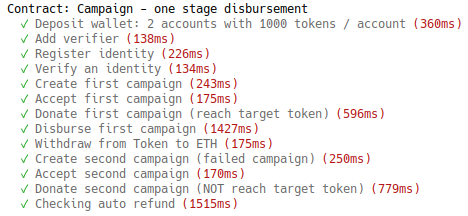
\includegraphics[scale=1]{result-one-stage}}
\caption{Kết quả kiểm thử kịch bản 1}
\end{center}
\end{figure}

Hình \ref{fig:result-multi-stage} là kết quả kiểm thử với kịch bản 2.

\begin{figure}[ht!]
\begin{center}
\label{fig:result-multi-stage}
\begin{tabular}{cc}
\fbox{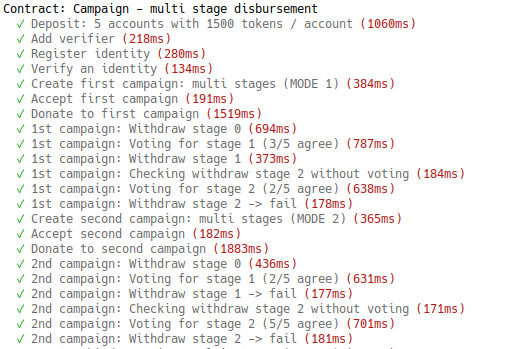
\includegraphics[scale=0.5]{result-multi-stage-1}}
&
\fbox{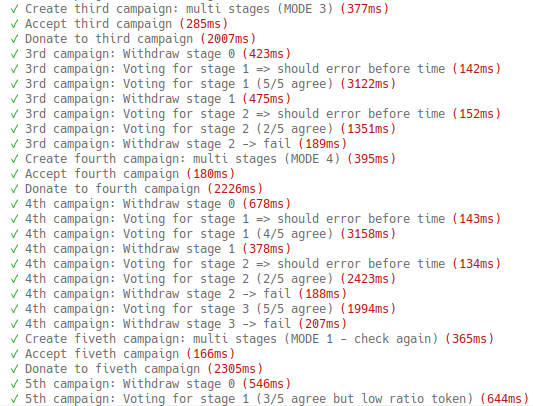
\includegraphics[scale=0.5]{result-multi-stage-2}}
\end{tabular}
\caption{Kết quả kiểm thử kịch bản 2}
\end{center}
\end{figure}

\subsection{Đo lường tốc độ thực hiện giao dịch}
Để tăng tính tin cậy cho phần đánh giá dưới đây của khóa luận, nhóm tác giả đã tham khảo mô hình đánh giá và kết quả đánh giá về hiệu suất của ethereum ở các công trình khác để làm thước đo và thực hiện tương tự với mô hình đánh giá đó.

Cụ thể, công trình của tác giả Sara Rouhani và Ralph Deters \cite{rouhani2017performance} đã đo được thời gian trung bình cho mỗi \gls{transaction} là 104.609ms với Parity client và 198.9125ms với Geth. Tổng số \gls{transaction} được gửi là 2000. Hai Ethereum private \gls{blockchain} khác nhau với cùng cấu hình được thực thi bởi Parity client và Geth client được sử dụng để đo lường. Cấu hình hệ thống bao gồm 24GB RAM và Core i7-6700 CPU. Việc gửi các \gls{transaction} được thực hiện bằng ngôn ngữ NodeJS và sau đó thu thập thời gian xử lí cho việc xác nhận các \gls{transaction}.

\subsubsection{Môi trường thực hiện đánh giá}
Nhóm tác giả thực hiện việc đánh giá này trên cấu hình máy như sau:

\begin{itemize}
\item \textbf{Chip xử lí}: 4 x Intel(E) Pentium(R) CPU N3540 @ 2.16GHz
\item \textbf{RAM}: 8GB
\item \textbf{Hệ điều hành}: Alpine Linux 3.9 chạy trên Docker container
\end{itemize}

Công cụ mà nhóm tác giả sử dụng trong phần đánh giá này là \textbf{Truffle framework}\footnote{https://www.trufflesuite.com}, đây là một bộ công cụ được sử dụng để triển khai các hợp đồng thông minh hỗ trợ ngôn ngữ Solidity.

Trong phần đánh giá thời gian này, nhóm tác giả sử dụng một mạng ethereum riêng được chạy trên mạng cục bộ nhằm loại bỏ đi thời gian chờ xác nhận giao dịch thông thường trên các mạng công khai hiện tại.

\subsubsection{Phương pháp thực hiện đánh giá}
Đầu tiên nhóm tác giả thực hiện lựa chọn các hàm trong hợp đồng thông minh thường xuyên được sử dụng trong hệ thống, sau đó các hàm được chọn sẽ được hiện thực thông qua các \gls{transaction}. Các \gls{transaction} sẽ được xử lí và gửi đi bằng NodeJS, thời gian đo được tính từ lúc \gls{transaction} được tạo ra đến lúc hoàn tất \gls{transaction} đó. Với mỗi \gls{transaction}, thực hiện gửi đi tuần tự 100, 200, 400, 600, 900 lần với cùng một bộ tham số cho trước. Sau đó lấy kết quả là thời gian trung bình thực hiện cho mỗi \gls{transaction}.

Các hàm được chọn và tham số đầu vào cho mỗi hàm để đo thời gian được thể hiện ở bảng \ref{tab:listfunction-timeperform}.

\begin{table}[!ht]
\centering
\resizebox{\textwidth}{!}{%
\begin{tabular}{|l|l|l|l|}
\hline
\multicolumn{1}{|c|}{\textbf{Contract}} & \multicolumn{1}{c|}{\textbf{Hàm được chọn}} & \multicolumn{1}{c|}{\textbf{Tham số đầu vào}}                                                                                                                                                                                                                           & \multicolumn{1}{c|}{\textbf{Ghi chú}}                    \\ \hline
Wallet                                  & deposit()                                   &                                                                                                                                                                                                                                                                         & \\ \hline
\multirow{3}{*}{Campaigns}              & createCampaign()                            & \begin{tabular}[c]{@{}l@{}}77760000,\\ 1000000,\\ 1,\\ {[}{]},\\ 0,\\ {[}{]},\\ '8f1ef45972ebd8ef45b2410e8a0b399181fed3d929738d2eb96baf470758a97d',\\ 'c2337a3217ffcf3b01398d83577a1c32235ceb4f481b8c7be00a055798e95d36'\end{tabular}                                   & \begin{tabular}[c]{@{}l@{}}một g.đoạn\\giải ngân\end{tabular}            \\ \cline{2-4} 
                                        & createCampaign()                            & \begin{tabular}[c]{@{}l@{}}77760000,\\ 1000000,\\ 3,\\ {[}300000, 300000, 400000{]}\\ 2,\\ {[}0, 7200, 7200{]},\\'8f1ef45972ebd8ef45b2410e8a0b399181fed3d929738d2eb96baf470758a97d',\\ 'c2337a3217ffcf3b01398d83577a1c32235ceb4f481b8c7be00a055798e95d36'\end{tabular} & \begin{tabular}[c]{@{}l@{}}nhiều g.đoạn\\giải ngân\end{tabular} \\ \cline{2-4} 
                                        & donate()                                    & \begin{tabular}[c]{@{}l@{}}0,\\ 1\end{tabular}                                                                                                                                                                                                                          &                                                          \\ \hline
\end{tabular}%
}
\caption{Các hàm và tham số đầu vào được dùng để đo thời gian thực hiện giao dịch}
\label{tab:listfunction-timeperform}
\end{table}

\subsubsection{Kết quả đánh giá}
Sau khi thực hiện đánh giá thời gian, nhóm tác giả đã tổng hợp kết quả như ở bảng \ref{tab:result-timeperform}. Theo như kết quả tổng hợp được, nhóm tác giả nhận xét rằng với dữ liệu đầu vào càng nhiều (kích thước lớn) thì thời gian xử lí càng lâu.

% Please add the following required packages to your document preamble:
% \usepackage{multirow}
% \usepackage{graphicx}
\begin{table}[!ht]
\centering
\resizebox{\textwidth}{!}{%
\begin{tabular}{|l|l|l|l|l|l|l|l|l|}
\hline
\multicolumn{1}{|c|}{\textbf{Contract}} & \multicolumn{1}{c|}{\textbf{Hàm}} & \multicolumn{1}{c|}{\textbf{\begin{tabular}[c]{@{}c@{}}Thời gian\\ thực hiện\\ 100 lần\\ (giây)\end{tabular}}} & \multicolumn{1}{c|}{\textbf{\begin{tabular}[c]{@{}c@{}}Thời gian\\ thực hiện\\ 200 lần\\ (giây)\end{tabular}}} & \multicolumn{1}{c|}{\textbf{\begin{tabular}[c]{@{}c@{}}Thời gian\\ thực hiện\\ 400 lần\\ (giây)\end{tabular}}} & \multicolumn{1}{c|}{\textbf{\begin{tabular}[c]{@{}c@{}}Thời gian\\ thực hiện\\ 600 lần\\ (giây)\end{tabular}}} & \multicolumn{1}{c|}{\textbf{\begin{tabular}[c]{@{}c@{}}Thời gian\\ thực hiện\\ 900 lần\\ (giây\end{tabular}}} & \multicolumn{1}{c|}{\textbf{\begin{tabular}[c]{@{}c@{}}Thời gian\\ trung bình\\ (giây)\end{tabular}}} & \multicolumn{1}{c|}{\textbf{Ghi chú}}                            \\ \hline
Wallet                                  & deposit                           & 11.099                                                                                                         & 18.035                                                                                                         & 36.484                                                                                                         & 54.166                                                                                                         & 86.968                                                                                                        & 0.095856                                                                                              &                                                                  \\ \hline
\multirow{3}{*}{Campaigns}              & createCampaign                    & 19.613                                                                                                         & 37.839                                                                                                         & 76.577                                                                                                         & 115.433                                                                                                        & 172.447                                                                                                       & 0.1921527                                                                                             & \begin{tabular}[c]{@{}l@{}}một g.đoạn\\ giải ngân\end{tabular}   \\ \cline{2-9} 
                                        & createCampaign                    & 31.986                                                                                                         & 63.561                                                                                                         & 127.236                                                                                                        & 191.94                                                                                                         & 287.694                                                                                                       & 0.319063                                                                                              & \begin{tabular}[c]{@{}l@{}}nhiều g.đoạn\\ giải ngân\end{tabular} \\ \cline{2-9} 
                                        & donate                            & 16.529                                                                                                         & 32.083                                                                                                         & 63.9                                                                                                           & 94.204                                                                                                         & 142.934                                                                                                       & 0.160255                                                                                              &                                                                  \\ \hline
\end{tabular}%
}
\caption{Bảng kết quả đánh giá thời gian hiện thực một số hàm trong hệ thống.}
\label{tab:result-timeperform}
\end{table}

Từ kết quả thu được, ta có biểu đồ tổng quan về tốc độ thực hiện của các hàm như ở hình \ref{fig:result-time-perform-chart}.

\begin{figure}[ht!]
\begin{center}
\label{fig:result-time-perform-chart}
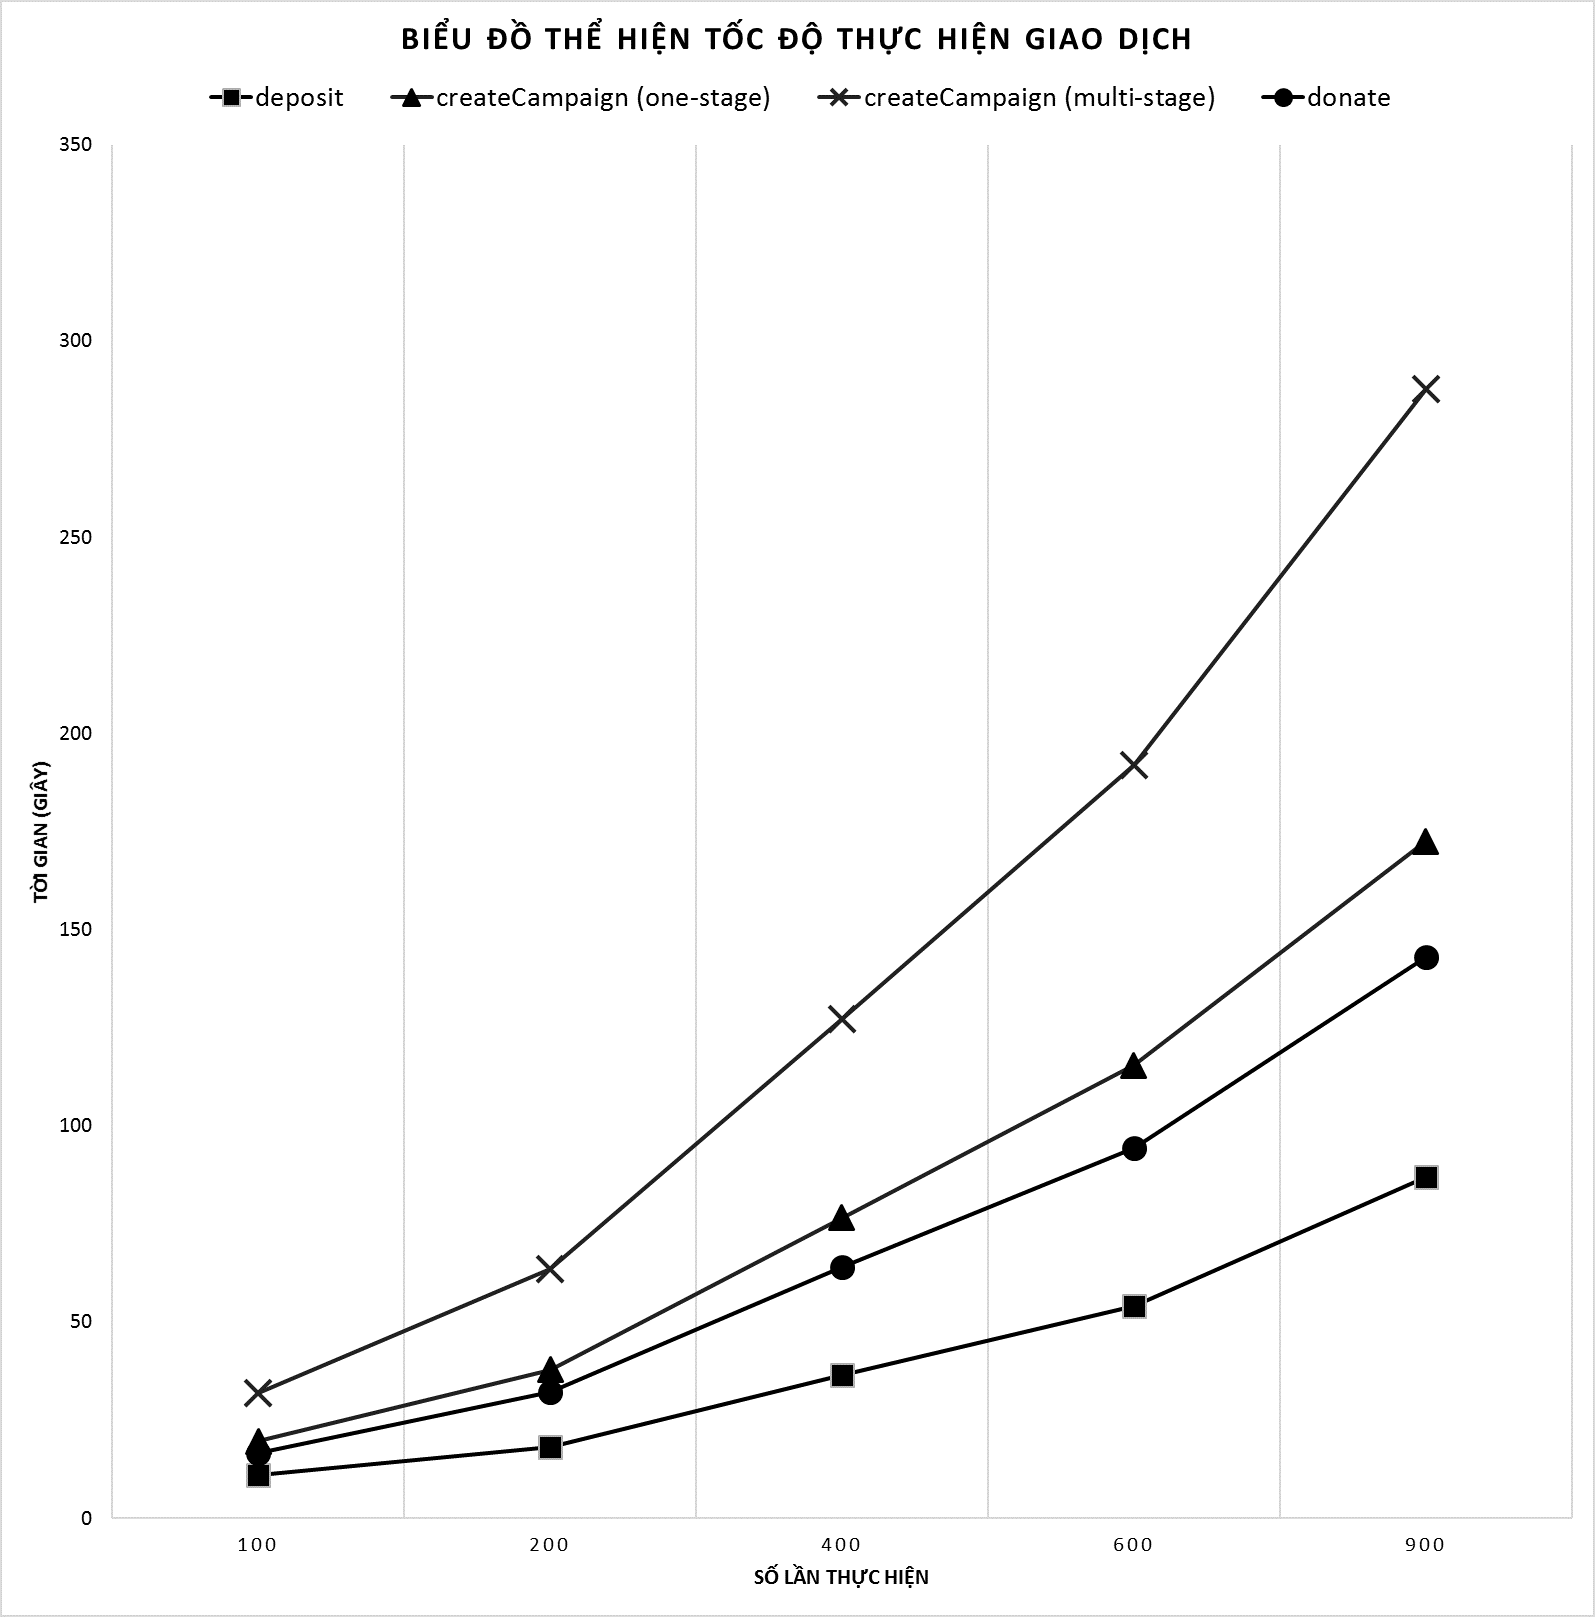
\includegraphics[scale=0.5]{result-time-perform-chart}
\caption{Biểu đồ thể hiện tốc độ thực hiện giao dịch giữa các hàm}
\end{center}
\end{figure}

Nhìn vào kết quả, ta thấy được:

\begin{itemize}
\item Hàm \textit{deposit} là hàm có tốc độ thực hiện nhanh nhất với thời gian trung bình là 0.095856 giây. Phần mã xử lí của hàm deposit tương đối ngắn nên thời gian xử lí nhanh hơn.
\item Hàm có tốc độ xử lí chậm nhất là hàm \textit{createCampaign} (với chiến dịch gây quỹ có nhiều giai đoạn giải ngân). Do hàm này có tham số đầu vào tương đối nhiều và phần mã xử lí phức tạp hơn nên thời gian hoàn tất lâu hơn những hàm khác.
\end{itemize}
\subsection{Chi phí thực hiện các giao dịch trong hệ thống}
\subsubsection{Môi trường thực hiện đánh giá}
Nhóm tác giả thực hiện việc đo lường chi phí giao dịch trên cấu hình máy như sau:

\begin{itemize}
\item \textbf{Chip xử lí}: 4 x Intel(E) Pentium(R) CPU N3540 @ 2.16GHz
\item \textbf{RAM}: 8GB
\item \textbf{Hệ điều hành}: Alpine Linux 3.9 running in Docker container
\end{itemize}

Bộ công cụ \textbf{Truffle framework} kết hợp plug-in có tên là \textbf{eth-gas-reporter}\footnote{https://www.npmjs.com/package/eth-gas-reporter} được sử dụng để triển khai các hợp đồng thông minh và đo lường chi phí thực hiện. Mạng ethereum riêng chạy trên máy cục bộ được sử dụng nhằm loại bỏ đi thời gian chờ xác nhận giao dịch thông thường trên các mạng công khai hiện tại.
\subsubsection{Phương pháp thực hiện đánh giá}
Do chỉ có các hàm thực hiện ghi dữ liệu mới tốn chi phí thực hiện nên nhóm tác giả chọn ra các hàm có thao tác ghi dữ liệu, sau đó các hàm được chọn sẽ được hiện thực thông qua các \gls{transaction}. Các \gls{transaction} sẽ được xử lí và gửi đi bằng NodeJS. Sau đó thực hiện ghi lại kết quả chi phí.

Các hàm được chọn và tham số đầu vào cho mỗi hàm để đo lường chi phí được thể hiện ở bảng \ref{tab:input-cost-perform}. Các tham số đầu vào mẫu được cho là sát với thực tế khi triển khai hệ thống (độ dài từng tham số mẫu là sát với thực tế).

\begin{table}[!ht]
\centering
\resizebox{\textwidth}{!}{%
\begin{tabular}{|l|l|l|l|}
\hline
\multicolumn{1}{|c|}{\textbf{Contract}} & \multicolumn{1}{c|}{\textbf{Hàm}} & \multicolumn{1}{c|}{\textbf{Dữ liệu đầu vào}}                                                                                                                                                                                                                                                                                                                                                  & \multicolumn{1}{c|}{\textbf{Ghi chú}}                                                                \\ \hline
\multirow{2}{*}{Wallet}                 & deposit                           &                                                                                                                                                                                                                                                                                                                                                                                                & \\ \cline{2-4} 
                                        & withdraw                          & 1000                                                                                                                                                                                                                                                                                                                                                                                           &                                                                                                      \\ \hline
\multirow{4}{*}{Identity}               & addVerify                         & \begin{tabular}[c]{@{}l@{}}'0x93598a39777ED4B4Af3Ac7429d123Ca3bE9658C5',\\ 'AAAAB3NzaC1yc2EAAAADAQABAAAAgQCDxbho2O3XWhktz4Hwi6/61ltfk/l\\ SCqeXLufvjr6O3wh1++MmTZT+KzcO0azsKsiFJTXL7ynC06Vp1Hp9o0BK3Q/Q\\ ZTo8jRoP3XX1LBu1CLe7OeOA5P2TO/nz2mWtuxz0b11GmRrjO8YoznizlPiolL\\ kv9hoDBvwTy0JonyJ6+w=='\end{tabular}                                                                                &                                                                                                      \\ \cline{2-4} 
                                        & changePubKey                      & \begin{tabular}[c]{@{}l@{}}'0x93598a39777ED4B4Af3Ac7429d123Ca3bE9658C5',\\ 'MIGfMA0GCSqGSIb3DQEBAQUAA4GNADCBiQKBgQCMjs5j52lzXN6XX+nZ1js\\ yaBgzVBsA/JlWVux1zL0pw4GocvqPsZrIKwKsTeQycGdf3azjKRKwMga6g8fPF\\ HO+Ayh+6v33B1h+3ckWu81alwsM+Y9ADpcMret5qH2Mv9rDyWi+lmAYeUA\\ OOosAWfmgc6QJz+psSMtuGKOr08q+1wIDAQAB'\end{tabular}                                                                    &                                                                                                      \\ \cline{2-4} 
                                        & registerIdentity                  & \begin{tabular}[c]{@{}l@{}}'KLTN',\\ 'UIT-HCM, Linh Trung, Thu Duc, HCM',\\ 830550240,\\ 'QmarHSr9aSNaPSR6G9KFPbuLV9aEqJfTk1y9B8pdwqK4Rq',\\ 'frPULs0boASMCqSq1guu+jX636wkY+fzhFSRnFQi9dQuK50yzCobUIGm5b/f7\\ oGDea/NrieB5c883EpWiQdgJlO+0B43jJLAtfSfJ/mlbGX3FUPc6LAQzxlCb5FSh\\ 7+Q1E4WIUyFwLwoNdipDYFcpuXxtCsKeepjFHwGFhfupxM=',\\ '0x93598a39777ED4B4Af3Ac7429d123Ca3bE9658C5'\end{tabular} &                                                                                                      \\ \cline{2-4} 
                                        & verify                            & \begin{tabular}[c]{@{}l@{}}'0x41A418C946Fd3201b7b2b30B367De35b0c54A6ce',\\ true\end{tabular}                                                                                                                                                                                                                                                                                                   &                                                                                                      \\ \hline
\multirow{7}{*}{Campaigns}              & createCampaign                    & \begin{tabular}[c]{@{}l@{}}77760000,\\ 1000000,\\ 1,\\ {[}{]},\\ 0,\\ {[}{]},\\ '8f1ef45972ebd8ef45b2410e8a0b399181fed3d929738d2eb96baf470758a97d',\\ 'c2337a3217ffcf3b01398d83577a1c32235ceb4f481b8c7be00a055798e95d36'\end{tabular}                                                                                                                                                          & \begin{tabular}[c]{@{}l@{}}một g.đoạn\\giải ngân\end{tabular}            \\ \cline{2-4} 
                                        & createCampaign                    & \begin{tabular}[c]{@{}l@{}}10,\\ 1000,\\ 3,\\ {[}300, 300, 400{]},\\ 0,\\ {[}{]},\\ '8f1ef45972ebd8ef45b2410e8a0b399181fed3d929738d2eb96baf470758a97d',\\ 'c2337a3217ffcf3b01398d83577a1c32235ceb4f481b8c7be00a055798e95d36'\end{tabular}                                                                                                                                                      & \begin{tabular}[c]{@{}l@{}}nhiều g.đoạn\\giải ngân\end{tabular} \\ \cline{2-4} 
                                        & verifyCampaign                    & \begin{tabular}[c]{@{}l@{}}1,\\ true\end{tabular}                                                                                                                                                                                                                                                                                                                                              &                                                                                                      \\ \cline{2-4} 
                                        & donate                            & \begin{tabular}[c]{@{}l@{}}1,\\ 1000\end{tabular}                                                                                                                                                                                                                                                                                                                                              &                                                                                                      \\ \cline{2-4} 
                                        & claimRefund                       & \begin{tabular}[c]{@{}l@{}}1,\\ 200\end{tabular}                                                                                                                                                                                                                                                                                                                                               &                                                                                                      \\ \cline{2-4} 
                                        & donate                            & \begin{tabular}[c]{@{}l@{}}1,\\ 200\end{tabular}                                                                                                                                                                                                                                                                                                                                               & \begin{tabular}[c]{@{}l@{}}donate lần 2\end{tabular}          \\ \cline{2-4} 
                                        & endCampaign                       & 1                                                                                                                                                                                                                                                                                                                                                                                              &                                                                                                      \\ \hline
Disbursement                            & vote                              & \begin{tabular}[c]{@{}l@{}}1,\\ 1,\\ true\end{tabular}                                                                                                                                                                                                                                                                                                                                         &                                                                                                      \\ \hline
\end{tabular}%
}
\caption{Các hàm và dữ liệu đầu vào được dùng để đo lường chi phí giao dịch}
\label{tab:input-cost-perform}
\end{table}

\subsubsection{Kết quả đo lường chi phí các giao dịch trong hệ thống}
Bảng tổng hợp chi phí cho các giao dịch được liệt kê ở bảng \ref{tab:result-cost-perform}. Kết quả màn hình khi chạy công cụ đo lường chi phí được thể hiện ở hình \ref{fig:result-perform-cost-1}.

\begin{figure}[ht!]
\begin{center}
\label{fig:result-perform-cost-1}
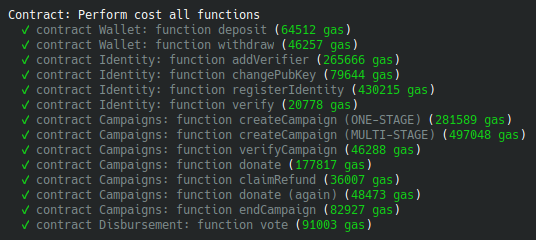
\includegraphics[scale=0.8]{result-perform-cost-1}
\caption{Ảnh chụp màn hình kết quả đo lường chi phí giao dịch}
\end{center}
\end{figure}

Công cụ đo lường còn cung cấp cho chúng ta chi phí triển khai các hợp đồng thông minh, kết quả được thể hiện ở bảng \ref{tab:result-cost-deployment}.

Một số đại lượng trong bảng kết quả:

\begin{itemize}
\item \textbf{Gas} - là một đơn vị đo lường công việc tính toán của các giao dịch hoặc hợp đồng thông minh trong mạng Ethereum.
\item \textbf{ETH} - là một đơn vị tiền tệ được sử dụng nội bộ trong mạng Ethereum. Tỉ lệ trao đổi giữa các đại lượng như sau: giá gas là 2 GWei/gas, và 1 ETH = $10^9$ GWei. Giá trị chuyển đổi giữa ETH và USD hiện tại được tham khảo trên \textbf{CoinMarketcap}\footnote{https://coinmarketcap.com} là 150.08 USD/ETH (cập nhật ngày 27/11/2019)
\end{itemize}

% Please add the following required packages to your document preamble:
% \usepackage{multirow}
\begin{table}[!ht]
\centering
\begin{tabular}{|l|l|l|l|l|}
\hline
\multicolumn{1}{|c|}{\textbf{Contract}} & \multicolumn{1}{c|}{\textbf{Hàm}} & \multicolumn{1}{c|}{\textbf{\begin{tabular}[c]{@{}c@{}}Chi phí\\ tính toán\\ (gas)\end{tabular}}} & \multicolumn{1}{c|}{\textbf{\begin{tabular}[c]{@{}c@{}}Chi phí\\ giao dịch\\ (ETH)\end{tabular}}} & \multicolumn{1}{c|}{\textbf{\begin{tabular}[c]{@{}c@{}}Chi phí\\ giao dịch\\ (USD)\end{tabular}}} \\ \hline
\multirow{2}{*}{Wallet}                 & deposit                           & 64512                                                                                             & 0.000129024                                                                                       & 0.02                                                                                              \\ \cline{2-5} 
                                        & withdraw                          & 46257                                                                                             & 0.000092514                                                                                       & 0.01                                                                                              \\ \hline
\multirow{4}{*}{Identity}               & addVerify                         & 265666                                                                                            & 0.000531332                                                                                       & 0.08                                                                                              \\ \cline{2-5} 
                                        & changePubKey                      & 79644                                                                                             & 0.000159288                                                                                       & 0.02                                                                                              \\ \cline{2-5} 
                                        & registerIdentity                  & 430215                                                                                            & 0.000860430                                                                                       & 0.13                                                                                              \\ \cline{2-5} 
                                        & verify                            & 20778                                                                                             & 0.000041556                                                                                       & 0.01                                                                                              \\ \hline
\multirow{7}{*}{Campaigns}              & createCampaign                    & 281589                                                                                            & 0.000563178                                                                                       & 0.08                                                                                              \\ \cline{2-5} 
                                        & createCampaign                    & 497048                                                                                            & 0.000994096                                                                                       & 0.15                                                                                              \\ \cline{2-5} 
                                        & verifyCampaign                    & 46288                                                                                             & 0.000092576                                                                                       & 0.01                                                                                              \\ \cline{2-5} 
                                        & donate                            & 177817                                                                                            & 0.000355634                                                                                       & 0.05                                                                                              \\ \cline{2-5} 
                                        & claimRefund                       & 36007                                                                                             & 0.000072014                                                                                       & 0.01                                                                                              \\ \cline{2-5} 
                                        & donate                            & 48473                                                                                             & 0.000096946                                                                                       & 0.01                                                                                              \\ \cline{2-5} 
                                        & endCampaign                       & 82927                                                                                             & 0.000165854                                                                                       & 0.02                                                                                              \\ \hline
Disbursement                            & vote                              & 91003                                                                                             & 0.000182006                                                                                       & 0.03                                                                                              \\ \hline
\end{tabular}
\caption{Kết quả đo lường chi phí giao dịch}
\label{tab:result-cost-perform}
\end{table}


\begin{table}[!ht]
\centering
\begin{tabular}{|l|l|l|l|}
\hline
\multicolumn{1}{|c|}{\textbf{Contract}} & \multicolumn{1}{c|}{\textbf{\begin{tabular}[c]{@{}c@{}}Chi phí\\ (gas)\end{tabular}}} & \multicolumn{1}{c|}{\textbf{\begin{tabular}[c]{@{}c@{}}Chi phí\\ (ETH)\end{tabular}}} & \multicolumn{1}{c|}{\textbf{\begin{tabular}[c]{@{}c@{}}Chi phí\\ (USD)\end{tabular}}} \\ \hline
Campaigns                               & 3447461                                                                               & 0.006894922                                                                           & 1.03                                                                                  \\ \hline
Disbursement                            & 1331555                                                                               & 0.002663110                                                                           & 0.4                                                                                   \\ \hline
Identity                                & 2401480                                                                               & 0.004802960                                                                           & 0.72                                                                                  \\ \hline
Wallet                                  & 1163284                                                                               & 0.002326568                                                                           & 0.35                                                                                  \\ \hline
\end{tabular}
\caption{Kết quả đo lường chi phí triển khai các hợp đồng}
\label{tab:result-cost-deployment}
\end{table}

Đánh giá tổng quan về chi phí:

\begin{itemize}
\item Hàm \textit{verify} trong contract Identity có mức chi phí thực hiện thấp nhất với 20778 gas (tương đương 0.000041556 ETH). Phần mã xử lí của hàm này tương đối ngắn nên chi phí thấp hơn.
\item Hàm có chi phí cao nhất là hàm \textit{createCampaign} (tạo chiến dịch với nhiều giai đoạn) với chi phí 497048 gas (tương đương 0.000994096 ETH). Do hàm này có tham số đầu vào tương đối nhiều và phần mã xử lí phức tạp hơn nên chi phí cao hơn những hàm khác.
\item Contract \textit{Campaigns} có chi phí triển khai cao nhất (3447461 gas), contract có chi phí triển khai thấp nhất là \textit{Identity} với 1163284 gas.
\end{itemize}
\subsection{Phân tích bảo mật của hợp đồng thông minh trong hệ thống}
\subsubsection{Các lỗ hổng phổ biến trong hợp đồng thông minh trên Ethereum}
Các lỗ hổng phổ biến được nhóm tác giả tham khảo từ công trình khảo sát của tác giả Nicola Atzei \cite{atzei2016survey}, bảng \ref{tab:smartcontract-vuln} là bảng tổng hợp được trình được trích dẫn từ tác giả Atzei.

% Please add the following required packages to your document preamble:
% \usepackage{multirow}
\begin{table}[!ht]
\centering
\begin{tabular}{|l|l|}
\hline
\multicolumn{1}{|c|}{\textbf{Level}} & \multicolumn{1}{c|}{\textbf{Cause of vulnerability}} \\ \hline
\multirow{6}{*}{Solidity} & Call to the unknown \\ \cline{2-2} 
 & Gasless send \\ \cline{2-2} 
 & Exception disorders \\ \cline{2-2} 
 & Type casts \\ \cline{2-2} 
 & Reentrancy \\ \cline{2-2} 
 & Keeping secrets \\ \hline
\multirow{3}{*}{EVM} & Immutable bugs \\ \cline{2-2} 
 & Ether lost in transfer \\ \cline{2-2} 
 & Stack size limit \\ \hline
\multirow{3}{*}{Blockchain} & Unpredictable state \\ \cline{2-2} 
 & Generating randomness \\ \cline{2-2} 
 & Time constraints \\ \hline
\end{tabular}
\caption{Bảng tổng hợp các lỗ hổng trong hợp đồng thông minh trên Ethereum \cite{atzei2016survey}.}
\label{tab:smartcontract-vuln}
\end{table}

Phần này chỉ tập trung vào giới thiệu các lỗi phổ biến với smart contract được lập trình bằng ngôn ngữ Solidity.

\textbf{Call to unknown} -- một lổ hổng khi gọi tới một vài lệnh cơ bản trong solidity như \texttt{call}, \texttt{send}, \texttt{delegatecall}. Nếu đối tượng được gọi trong các hàm này không tồn tại thì sẽ có một tác dụng phụ là gọi đến hàm fallback\footnote{fall back là một hàm đặc biệt trong smart contract, là hàm không có tên và được sử dụng khi: contract nhận ether, hoặc khi có ai đó gọi hàm không có trong contract hoặc tham số không đúng.} của người nhận.

\textbf{Gasless send} -- khi sử dụng hàm \texttt{send} để chuyển \gls{eth} sang contract, có thể xảy ra lỗi out-of-gas (hết gas / không đủ gas) do việc thực thi hàm \texttt{send} đến contract sẽ dẫn đến gọi fallback của contract, mà số gas giới hạn trong trường hợp này là 2300 gas. Mà 2300 gas chỉ cho phép thực hiện một tập bytecode giới hạn, ví dụ: những lệnh / hàm không làm thay đổi trạng thái của contract. Nếu fallback có những tập lệnh phức tạp sẽ dẫn đến lỗi, khi đó người dùng sẽ bị mất toàn bộ phí thực hiện transaction.

\textbf{Exception disorder} -- có thể tạm dịch lỗ hổng này là làm rối exception. Trong smart contract có một điều đặc biệt là với một exception được ném ra thì sẽ có hai cách xử lí khác nhau phụ thuộc vào cách các contract gọi nhau. Cụ thể:

\begin{itemize}
\item Nếu tất cả lời gọi hàm trong chuỗi đều là lời gọi trực tiếp, thì việc thực thi dừng lại và mọi giá trị trong lúc thực thi được hoàn nguyên.
\item Nếu có ít nhất một lời gọi hàm được thực hiện thông qua lệnh \texttt{call} (tương tự với  \texttt{delegatecall} và \texttt{send}), thì exception được truyền dọc theo chuỗi, chỉ hoàn nguyên các giá trị thực thi bên trong hàm của lời gọi call. Từ thời điểm đó (từ lệnh \texttt{call}), việc thực hiện được nối lại, và lệnh \texttt{call} trả về \texttt{false}.
\end{itemize}

Để hiểu rõ về lỗ hổng, ta xem xét một ví dụ sau:

\begin{lstlisting}
contract Alice { function ping(uint) returns (uint) }

contract Bob { 
    uint x=0;
    function pong(Alice c) {
        x=1;
        c.ping(42);
        x=2;
    }
}
\end{lstlisting}

Có hai trường hợp xảy ra:

\begin{itemize}
\item Trường hợp 1: thực hiện gọi hàm pong của Bob và sau đó hàm ping của Alice ném ra một exception. Sau đó, việc thực thi dừng lại và các giá trị của toàn bộ giao dịch được hoàn nguyên. Do đó, biến \texttt{x} có giá trị là $0$ sau khi kết thúc việc thực thi.
\item Trường hợp 2: giả sử contract Bob gọi ping của Alice thông qua lệnh call và sau đó ping của Alice ném ra một exception. Khi đó, chỉ có giá trị bên trong hàm ping được hoàn nguyên và lúc này khi kết thúc việc thực thi thì giá trị của \texttt{x} là $2$.
\end{itemize}

Sự bất thường trong cách xử lý các trường hợp exception có thể ảnh hưởng đến tính bảo mật của contract. Chẳng hạn, sẽ khiến lập trình viên tin rằng việc chuyển ether thông qua hàm \texttt{send} là thành công chỉ vì không có exception nào có thể dẫn đến các cuộc tấn công.

\textbf{Type casts} -- trình biên dịch Solidity có thể phát hiện một số lỗi kiểu dữ liệu. Ví dụ: gán một giá trị số nguyên cho một biến thuộc kiểu chuỗi. Khi thực hiện gọi một hàm hay chương trình con nào đó, người gọi phải khai báo interface của hàm hay chương trình con đó. Nhưng điều này chỉ kiểm tra được hàm đó có tồn tại không, chứ không xác định được mã thực thi của hàm đích có trùng khớp với hàm thực tế cần gọi hay không. Do đó, điều này có thể đánh lừa lập trình vì khi thực thi sẽ không có bất lỗi nào được ném ra dù cho việc gọi hàm không đúng như mong muốn.

\textbf{Reentrancy} -- lỗ hổng này cho phép gọi lại một hàm không đệ quy lần nữa nhờ vào cơ chế gọi fallback của solidity. Như đã đề cập trước đó, nếu ta sử dụng lệnh call hoặc các lệnh tương tự mà đích đến không tồn tại hoặc rỗng thì sẽ thực hiện gọi fallback của contract, điều này có thể dẫn đến vòng lặp, vòng lặp này kết thúc khi tiêu thụ hết gas. Để rõ hơn lỗ hổng này, xem xét ví dụ sau:

\begin{lstlisting}
contract Bob {
  bool sent = false;
  function ping(address c) {
    if (!sent) {
      c.call.value(2)();
      sent = true;
    }
  }
}

contract Attacker {
  function() {
    Bob(msg.sender).ping(this);
  }
}
\end{lstlisting}

Cách khai thác ví dụ trên:

\begin{itemize}
\item Chức năng của hàm ping trong contract \textbf{Bob}: gửi 2wei đến địa chỉ \textbf{c}, sử dụng lệnh \texttt{call} có đích đến rỗng (tức không gọi hàm nào) và không có giới hạn gas.
\item Bây giờ, giả sử rằng ping đã được gọi với địa chỉ của \textbf{Attacker}. Như đã đề cập trước đó, \texttt{call} có tác dụng phụ là gọi fallback của \textbf{Attacker}, lần lượt gọi lại ping. Vì biến \textbf{sent} chưa được đặt thành \texttt{true}, Bob gửi lại 2wei cho Attacker và gọi lại fallback lần nữa, do đó bắt đầu một vòng lặp. Vòng lặp này kết thúc khi việc thực thi cuối cùng hết gas hoặc khi đạt đến giới hạn ngăn xếp hoặc khi Bob đã rút hết ether của mình.
\end{itemize}

\textbf{Keeping secrets} -- trong smart contract hỗ trợ việc khai báo cấp độ truy xuất dữ liệu từ riêng tư đến công khai. Tuy nhiên việc khai báo một biến hay một hàm nào đó là riêng tư chỉ có tác dụng ngăn người dùng hoặc contract khác gọi trực tiếp, trên thực tế người dùng vẫn đọc được giá trị của các biến được khai báo là riêng tư trong smart contract, do đó không đảm bảo được độ bí mật của dữ liệu. Điều này là do mỗi lời gọi hàm được đóng gói trong transaction, và các transaction này được công khai trong toàn mạng blockchain. Vì thế, mọi người đều có thể kiểm tra nội dung của giao dịch và suy ra giá trị của các trường dữ liệu.

\subsubsection{Các công cụ phân tích bảo mật smart contract}
\label{sec:smartcontract-vuln}
Danh sách các công cụ phân tích, đánh giá smart contract giới thiệu bên dưới được tham khảo từ công trình của tác giả Jiaming Ye \cite{8728953} và luận văn thạc sĩ của tác giả Ardit Dika \cite{dika2017ethereum}.

\textbf{Smartcheck}\footnote{https://tool.smartdec.net} -- là một công cụ phân tích tĩnh giúp phát hiện ra những lỗi hoặc cảnh báo trong smart contract được viết bằng Solidity. Công cụ này có các ưu điểm sau:

\begin{itemize}
\item Giao diện dễ sử dụng, kiểm tra được nhiều contract.
\item Các lỗ hổng có thể phát hiện: \textit{Non-strict comparison with zero}, \textit{Hardcoded address},  \textit{DoS by external contract}, \textit{Reentrancy}, \textit{Overflow and Underflow in Solidity}, \textit{Redundant fallback function}, \ldots.
\item Ở mỗi lỗi được phát hiện, smartcheck cung cấp cụ thể số dòng bị lỗi và đánh dấu chúng.
\item Bên cạnh việc phát hiện lỗ hổng, smartcheck còn cung cấp giải pháp khắc phục từng lỗ hổng đó.
\end{itemize}

\textbf{Remix}\footnote{https://remix.ethereum.org} -- là một IDE dựa trên web để phát triển hợp đồng thông minh. Ngoài ra, Remix IDE còn được sử dụng như một công cụ phân tích mã bảo mật để kiểm tra các lỗ hổng có thể xảy ra. Remix IDE chỉ được sử dụng để phân tích mã nguồn Solidity. Remix IDE có khả năng phân tích gần như 100\% các lỗ hổng hiện tại của hợp đồng thông minh \cite{dika2017ethereum}.

\textbf{Slither}\footnote{https://github.com/crytic/slither} -- là framework phân tích tĩnh Solidity được viết bằng Python 3. Slither chạy bộ các trình phát hiện lỗ hổng, in thông tin trực quan về chi tiết hợp đồng và cung cấp API để dễ dàng viết các phân tích tùy chỉnh. Slither cho phép các nhà phát triển tìm ra các lỗ hổng, tăng cường khả năng đọc mã và nhanh chóng phân tích với những sự tùy chỉnh. Các chức năng và ưu điểm của Slither:

\begin{itemize}
\item Phát hiện các lỗ hổng trong Solidity.
\item Xác định nơi xảy ra tình trạng lỗi trong mã nguồn.
\item Dễ dàng tích hợp với bộ công cụ Truffle.
\item Tích hợp các trình báo cáo để biểu diễn thông tin contract.
\item Hỗ trợ API để viết các trình phân tích tùy chỉnh bằng Python.
\item Khả năng phân tích các hợp đồng được viết với phiên bản Solidity > 0.4
\item Phân tích chính xác 99,9\% tất cả mã Solidity công khai.
\item Thời gian thực hiện trung bình dưới 1 giây mỗi contract.
\end{itemize}

Cả ba công cụ được giới thiệu ở trên đều là phần mềm mã nguồn mở.
\subsubsection{Kết quả phân tích}
Nhóm tác giả sử dụng các công cụ đã được giới thiệu ở mục \ref{sec:smartcontract-vuln} để thực hiện phân tích trên các smart contract của hệ thống. Cụ thể kết quả với từng công cụ như sau:

Kết quả phân tích với Remix IDE được thể hiện ở hình \ref{fig:result-remix-ide}. Kết quả công cụ phân tích của Remix chỉ đưa ra 5 cảnh báo, cụ thể ở cảnh báo đầu tiên là về việc sử dụng lệnh \texttt{send} để chuyển ether, thì nhóm tác giả đã kiểm tra kĩ lưỡng các giá trị trước và sau lệnh send này nên hạn chế được các lỗ hổng như reentrancy.

\begin{figure}[ht!]
\begin{center}
\label{fig:result-remix-ide}
\fbox{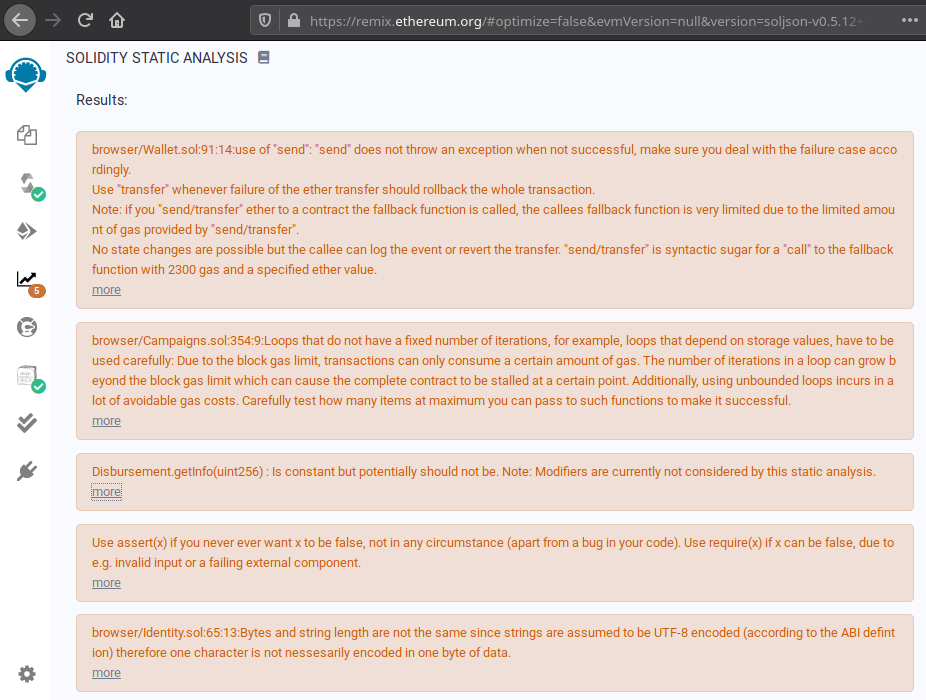
\includegraphics[scale=0.6]{result-remix-ide}}
\caption{Kết quả phân tích hợp đồng thông minh với Remix IDE}
\end{center}
\end{figure}

Hình \ref{fig:result-slither} là kết quả khi thực hiện phân tích với công cụ Slither. Kết quả phân tích cho thấy số contract thực hiện quét là 6 với 40 bộ nhận diện và có 3 vấn đề được tìm thấy. Các vấn đề quét được là cảnh báo lỗ hổng Reentrancy, tuy nhiên cảnh báo này không ảnh hướng đến bảo mật của contract.

\begin{figure}[ht!]
\begin{center}
\label{fig:result-slither}
\fbox{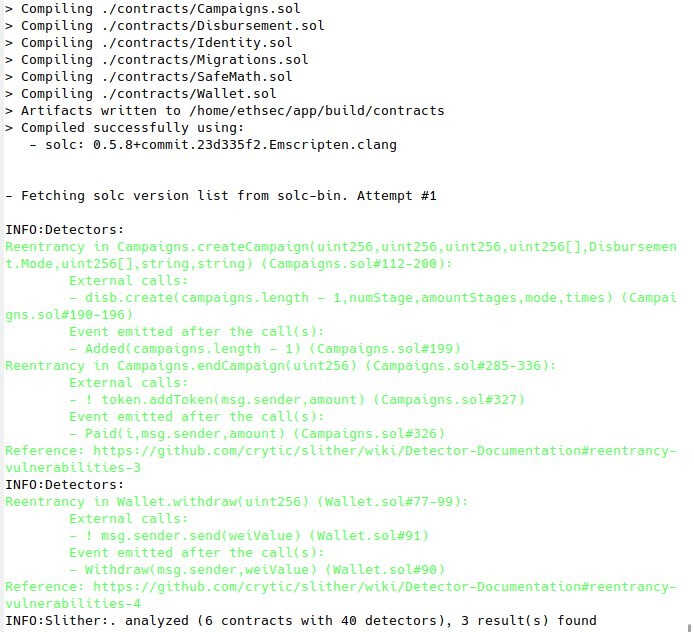
\includegraphics[scale=0.8]{result-slither}}
\caption{Kết quả phân tích hợp đồng thông minh với Slither}
\end{center}
\end{figure}

Công cụ Smartcheck được cung cấp dưới dạng giao diện web, do đó kết quả phân tích trên Smartcheck cũng được công khai\footnote{Kết quả phân tích với Smartcheck: https://tool.smartdec.net/scan/e6d6a5d37015403faf92395ec7f543c8}. Hình \ref{fig:result-smartcheck} là ảnh chụp kết quả phân tích các hợp đồng thông minh trong hệ thống trên trang Smartcheck. Trong kết quả ta thấy bên cột bên phải là danh sách các lỗi, đọc qua các lỗi thì đây là những cảnh báo giúp cho lập trình hiệu quả hơn, không ảnh hướng tới bảo mật của hợp đồng thông minh.

\begin{figure}[ht!]
\begin{center}
\label{fig:result-smartcheck}
\fbox{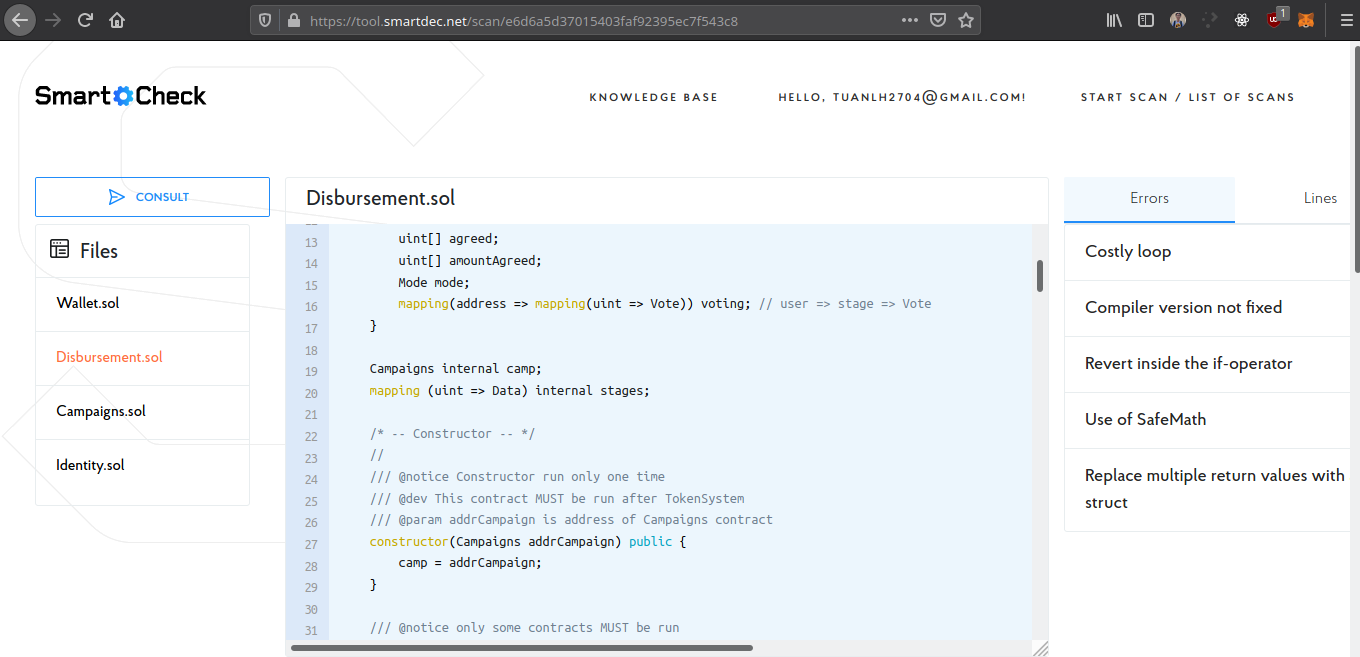
\includegraphics[scale=0.4]{result-smartcheck}}
\caption{Kết quả phân tích hợp đồng thông minh với Smartcheck}
\end{center}
\end{figure}

Đánh giá chung kết quả phân tích cho thấy, hợp đồng thông minh được hiện thực của hệ thống không gặp phải vấn đề bảo mật nghiêm trọng trên các công cụ đã phân tích.

\subsection{Đánh giá tốc độ tải trang của giao diện người dùng}
\subsubsection{Môi trường thực hiện}
Thông tin cấu hình máy sử dụng để đo tốc độ truy xuất của ReactJS như sau:

\begin{itemize}
\item Chip xử lý: 2.7 Ghz Dual-Core intel Core i5
\item Hệ điều hành: macOS Catalina version 10.15.1
\item RAM: 8GB 1867Mhz DDR3
\item Đồ họa: Intel Iris Graphics 6100 1536 MB
\item Trình duyệt Google Chrome version 78.0.3904 (được cài sẵn extension MetaMask đã cấp phép truy cập thông tin)
\end{itemize}
\subsubsection{Kết quả đánh giá}
Kết quả được tổng hợp ở bảng \ref{tab:result-perform-ui}.

% Please add the following required packages to your document preamble:
% \usepackage{graphicx}
\begin{table}[!ht]
\centering
\resizebox{\textwidth}{!}{%
\begin{tabular}{|l|l|l|l|l|l|l|l|}
\hline
\multicolumn{1}{|c|}{\textbf{Page}} & \multicolumn{1}{c|}{\textbf{Loading}} & \multicolumn{1}{c|}{\textbf{Scripting}} & \multicolumn{1}{c|}{\textbf{Rendering}} & \multicolumn{1}{c|}{\textbf{Painting}} & \multicolumn{1}{c|}{\textbf{System}} & \multicolumn{1}{c|}{\textbf{Idle}} & \multicolumn{1}{c|}{\textbf{Total}} \\ \hline
Detail campaign                     & 28 ms                                 & 1320 ms                                 & 70 ms                                   & 65 ms                                  & 220 ms                               & 918 ms                             & 2621 ms                             \\ \hline
Home page                           & 6 ms                                  & 743 ms                                  & 3 ms                                    & 3 ms                                   & 41 ms                                & 102 ms                             & 898 ms                              \\ \hline
Create campaign                     & 24 ms                                 & 1181 ms                                 & 47 ms                                   & 36 ms                                  & 196 ms                               & 672 ms                             & 2156 ms                             \\ \hline
Explore campaigns                   & 14 ms                                 & 798 ms                                  & 98 ms                                   & 82 ms                                  & 237 ms                               & 1541 ms                            & 2770 ms                             \\ \hline
\end{tabular}%
}
\caption{Bảng kết quả đo tốc độ truy xuất front-end của hệ thống}
\label{tab:result-perform-ui}
\end{table}

Đánh giá kết quả như sau:

\begin{itemize}
\item Trang danh sách chiến dịch (Explore campaign) có tổng thời gian hoàn thành lâu nhất với 2.77 giây, do trang này tải thông tin của nhiều chiến dịch, mỗi chiến dịch là một lời gọi đến hợp đồng thông minh. Bên cạnh đó, mỗi chiến dịch cũng cần truy xuất thông tin đến cơ sở dữ liệu tập trung. Thật vậy vì tốc độ tải ban đầu (cột ``loading'') tương đối thấp, do đó tổng thời gian hoàn thành trang lâu nhất là do ảnh hưởng các thành phần phụ thuộc kèm theo như đã đề cập.
\item Trang chủ (Home page) có thời gian hoàn thành nhanh nhất với 0.898 giây, không lạ gì do trang chủ hoàn toàn là một trang tĩnh.
\end{itemize}
\end{document}